\documentclass{article}
\usepackage{graphicx} % Required for inserting images
\usepackage{amsmath}
\usepackage{amssymb}
\usepackage{bbm}
\usepackage{hyperref}
\usepackage{titling}
\usepackage{fancyhdr} % to change header and footers
\graphicspath{ {./images/} }
\usepackage{marginnote}
\usepackage{tikz, pgfplots}
% \usetikzlibrary{positioning}
\pgfplotsset{compat=1.18}
\usetikzlibrary{automata,arrows,positioning,calc}


%\usepackage[left=1.0in,top=1.0in,right=1.0in,bottom=1.0in]{geometry} % Document margins

% \setlength{\droptitle}{-12em}   % This is your set screw
% Turn on the style
\pagestyle{fancy}
% Clear the header and footer
\fancyhead{}
\fancyfoot{}
% Set the right side of the footer to be the page number
\fancyfoot[R]{\thepage}

\title{MIT 6.041}
\author{Michael Mellinger \\ \href{mailto:mmellinger66@gmail.com}{mmellinger66@gmail.com} }
%\date{}

% === Tricks ===
% https://youtu.be/7B7ytLrMTa0
% \quad
% \qquad
% \hspace{1in}
% Text here. \hfill Push me to the right

% Naturals, reals, etc.
\newcommand{\N}{\mathbb{N}}
\newcommand{\Z}{\mathbb{Z}} 
\newcommand{\Q}{\mathbb{Q}}
\newcommand{\I}{\mathbb{I}}
\newcommand{\R}{\mathbb{R}}
\newcommand{\C}{\mathbb{C}}

\newcommand{\e}[1]{{\mathbb E}\left[ #1 \right]}
% https://stats.meta.stackexchange.com/questions/1419/latex-macros-for-expectation-variance-and-covariance
% \DeclareMathOperator{\E}{\mathbb{E}} \E(X,Y) 

\begin{document}

\maketitle
\tableofcontents
\clearpage

\section{Lecture 1: Probability Models and Axioms}

\marginpar{\href{https://youtu.be/j9WZyLZCBzs}{Video}} Read sections: 1.1, 1.2\\
\marginpar{\href{https://ocw.mit.edu/courses/6-041sc-probabilistic-systems-analysis-and-applied-probability-fall-2013/pages/unit-i/lecture-1/}{Lecture Home}}
\marginpar{\href{https://ocw.mit.edu/courses/6-041sc-probabilistic-systems-analysis-and-applied-probability-fall-2013/resources/mit6_041scf13_l01/}{Slides}}


\subsection{Sample Space - \texorpdfstring{$\Omega$}{Omega}}

\begin{figure}[h]
\centering
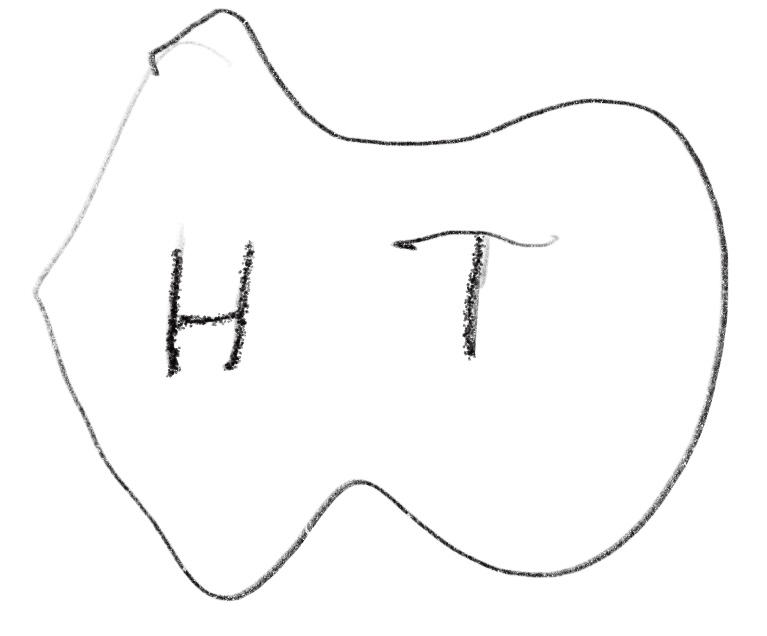
\includegraphics[width=5cm, height=4cm]{images/L01/IMG_1_1455.jpeg}
\caption{Missing}
\end{figure}

\begin{itemize}
    \item Sample space is a set
    \item Elements are the possible outcomes of the experiment
    \item Mutually exclusive
    \item Collectively exhaustive
\end{itemize}

\subsection{Example: 2 rolls of 4-sided die (tetrahedral die)}

% \reversemarginpar
\marginpar{(15:19)}
The experiment is both rolls (not 2 experiments)
% {(15:19)}

% 
\begin{figure}[ht]
\centering

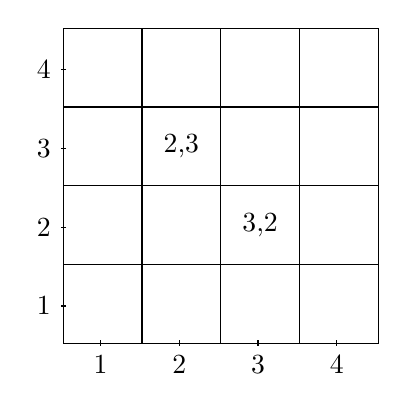
\begin{tikzpicture}
% \begin{axis}[
%     title={Unit Square},
%    height=8cm,width=8cm, 
%     xlabel={First Die},
%     x\ylabel={Second Die},
% ]
\draw (0,0) rectangle (4,4);
\draw (0,0) grid (4,4);
\foreach \x in {1,2,3,4}
   \draw[xshift=-15pt] (\x cm,1pt) -- (\x cm,-1pt) node[anchor=north] {$\x$};
\foreach \y in {1,2,3,4}
    \draw[yshift=-15pt] (1pt,\y cm) -- (-1pt,\y cm) node[anchor=east] {$\y$};

\draw (1.5,2.5) node{2,3};
\draw (2.5,1.5) node{3,2};
% \end{axis}
\end{tikzpicture}
\caption{2 4-Sided Die Roll Sample Space}
\end{figure}


Reserving the word "outcome" for the outcome of the overall experiment.

\subsection{Sequential Description}

\begin{figure}[ht]
\centering
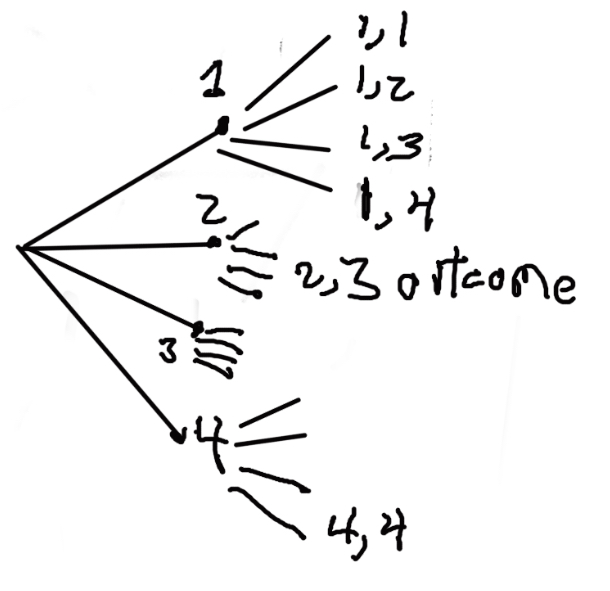
\includegraphics[width=5cm, height=4cm]{images/L01/sequential_desc.jpeg}
\caption{Sequential Description}
\end{figure}

\subsection{Sample Space: Continuous Example: Darts}

$\Omega = \{(x,y) | \quad 0 \le x, \quad y \le 1 \}$

\begin{figure}[ht]
\centering
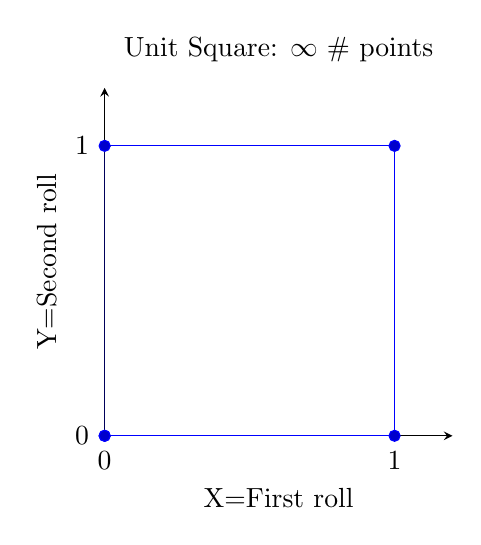
\begin{tikzpicture}
\begin{axis}[
    title={Unit Square: $\infty$ \# points},
   height=6cm,width=6cm, 
    axis lines = left,
    xmin=0, xmax=1.2,
    ymin=0, ymax=1.2,
    xlabel = \(x\),
    ylabel = {\(y\)},   
    xtick={0,1},
    ytick={0,1},
    xlabel={X=First roll},
    ylabel={Y=Second roll}
]
\addplot coordinates {
    (0,0)
    (0,1)
    (1,1)
    (1,0)
  (0,0)
     
};
\end{axis}
\end{tikzpicture}
\caption{Unit Square}
\end{figure}
We assign probabilities to the outcomes (not exactly).  Any individual point is zero.
\\
When we talk about the \textit{subsets} of sample space, we call them \textbf{events}.

\begin{figure}[ht]
\centering
    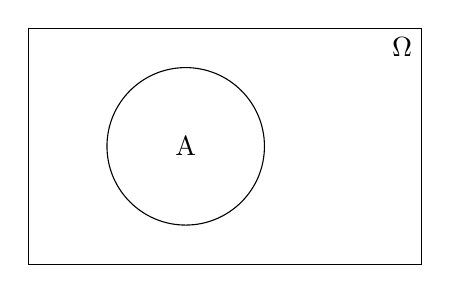
\begin{tikzpicture}
\draw (0,0) rectangle (5,3) node[anchor=north east] {$\Omega$};
\draw (2,1.5) circle (1cm) node {A};
\end{tikzpicture}
\caption{$\Omega$} \label{fig:M1}
\end{figure}


\subsection{Probability Axioms}

\begin{enumerate}
    \item Nonnegativity: \colorbox{yellow}{$P(A) > 0$}
    \item Normalization: $P(\Omega)=1$
    \item Additivity: If $A \cap B = \varnothing$, then $P(A \cup B)=P(A) + P(B)$
\end{enumerate}

\begin{figure}[!ht]
\centering
\begin{tikzpicture}
\draw (0,0) rectangle (7,4);
\draw (2,2) circle (1cm) node {A};
\draw (5,2) circle (1cm) node {B};
\end{tikzpicture}
\caption{A,B} \label{fig:M2}
\end{figure}

\begin{align*}
1 = P(\Omega) = \underbrace{P(A \cup A^c)}_{Cool stuff} \qquad \text{(by 2)}\\
= P(A) + P(A^c)  \qquad \text{(by 3)}\\
P(A) = 1 - P(A^c) \le 1  \qquad \text{(by 1)}\\
\end{align*}

Probabilities are always $\le 1$

\subsection{3 Events Union}

MISSING

\begin{figure}[!ht]
\centering
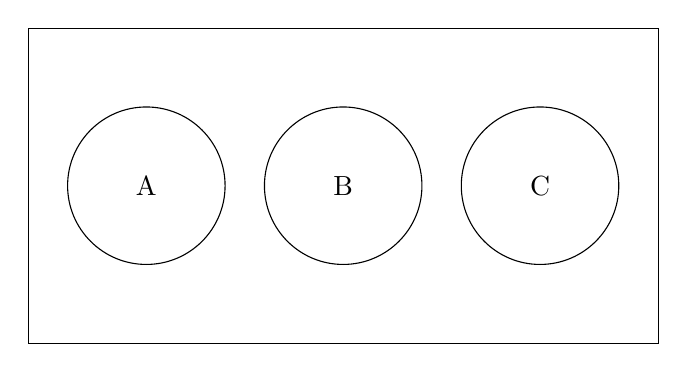
\begin{tikzpicture}
\draw (0,0) rectangle (8,4);
\draw (1.5,2) circle (1cm) node {A};
\draw (4,2) circle (1cm) node {B};
\draw (6.5,2) circle (1cm) node {C};
\end{tikzpicture}
\caption{A,B,C} \label{fig:M3}
\end{figure}

If $A_1,\ldots, A_n$ are disjoint then $P(A_1 \cup \cdots \cup A_n) = P(A_1) + \cdots + P(A_n)$

\begin{itemize}
    \item Axiom 3 has some issues \marginpar{(36:00)}
    \item Weird subsets.  Will ignore in this class.
\end{itemize}

\subsection{Discrete Uniform Law}

Model obeys this law if all outcomes are equally likely. (e.g. fair coins, fair dice, well-shuffled decks)

\subsection{Continuous Uniform Law}

\begin{figure}[!ht]
\centering
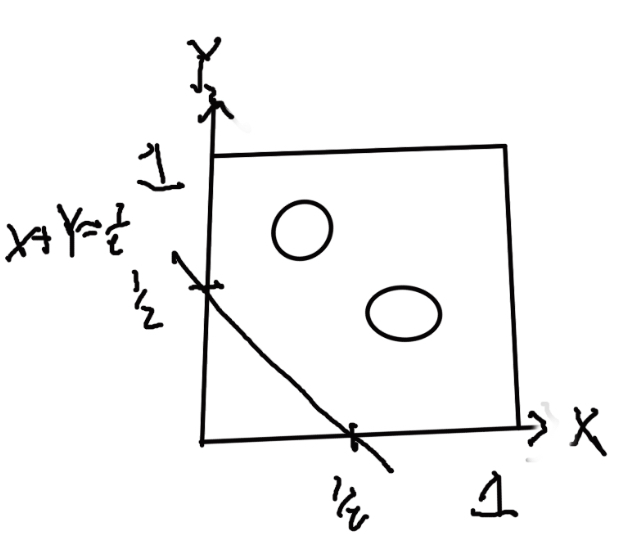
\includegraphics[width=5cm, height=4cm]{images/L01/cont_unif_law.jpeg}
\caption{x+y=1/2}
\end{figure}

\subsubsection{Uniform Law: Probability = Area}

\begin{align*}
P(X+Y \le \frac{1}{2}=? = \frac{1}{2} \frac{1}{2}\frac{1}{2} = \frac{1}{8}\frac{1}{2}b\cdot h\\
P((X,Y) = 0.5.0.3))= ? = 0 = \text{No area}
\end{align*}





\subsection{Example: Probability Law}

Countably infinite sample space.

equal areas = equal probabilities

\subsection{Countable Additivity Axiom}

If $A_1,\ldots, A_n$ are disjoint events, then can be arranged in order:

$$
P(A_1 \cup A_2 \cup \cdots) = P(A_1) + P(A_2) + \cdots
$$
Sequence of disjoint sets.


\section{Lecture 2: Conditioning and Bayes' Rule}

\marginpar{\href{https://youtu.be/TluTv5V0RmE}{Video}} Read sections: 1.3, 1.4\\
\marginpar{\href{https://ocw.mit.edu/courses/6-041sc-probabilistic-systems-analysis-and-applied-probability-fall-2013/pages/unit-i/lecture-2/}{Lecture Home}}
\marginpar{\href{https://ocw.mit.edu/courses/6-041sc-probabilistic-systems-analysis-and-applied-probability-fall-2013/a1462fa23de9d08c0dfd233a57278fed_MIT6_041SCF13_L02.pdf}{Slides}}

Example where countability axiom does not apply: We are not dealing with a \textit{sequence of sets}.

Zero probability doesn't mean impossible, just extremely unlikely by itself.

Expect the unexpected (10m)

$P(X)=1$ also doesn't mean certain.  "Essential certainty"

The issue is with continuous models.

\subsection{Conditional Probabilities}

\begin{figure}[ht]
\centering
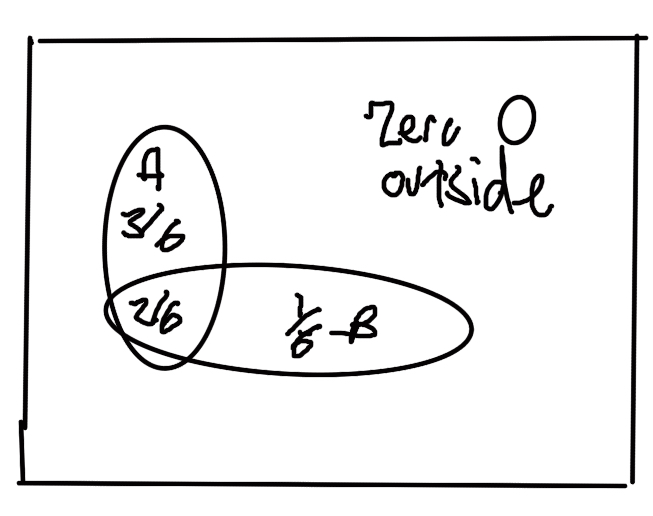
\includegraphics[width=10cm, height=7cm]{images/L02/cond_prob.jpeg}
\caption{Conditional Probabilities}
\end{figure}

$\frac{2}{6}$ is twice as likely as $\frac{1}{6}$. Want to keep proportion (16m)

$P(A|B)=$ Probability of A, given that B occurred.  B is our new universe.

\subsubsection{Definition}

$$
P(A|B) = \frac{P(A \cap B)}{P(B)}, \qquad \text{Assuming} P(B) \ne 0
$$

$$
\frac{2/6}{3/6} = \frac{2}{3}
$$

\marginpar{(17:30)} Can rewrite:
$$
P(A \cap B) = P(A \mid B)P(B) = P(B \mid A)P(A), \text{symmetrical relationship} 
$$

\marginpar{(19m)} These conditional probabilities are just probabilities and satisfy axioms.

\begin{align*}
A \cap B = \varnothing\\
P(A \cup B) = P(A) + P(B)
\end{align*}

Now we are placed in a universe where C occurred.

\begin{align*}
P(A \cup B \mid C) = P(A \mid C) + P(B \mid C)
\end{align*}

\subsection{Example: Dice Roll}

\marginpar{(23m)} The shortcut answer: Start with Uniform distribution, still uniform after we condition.

\begin{figure}[!ht]
\centering
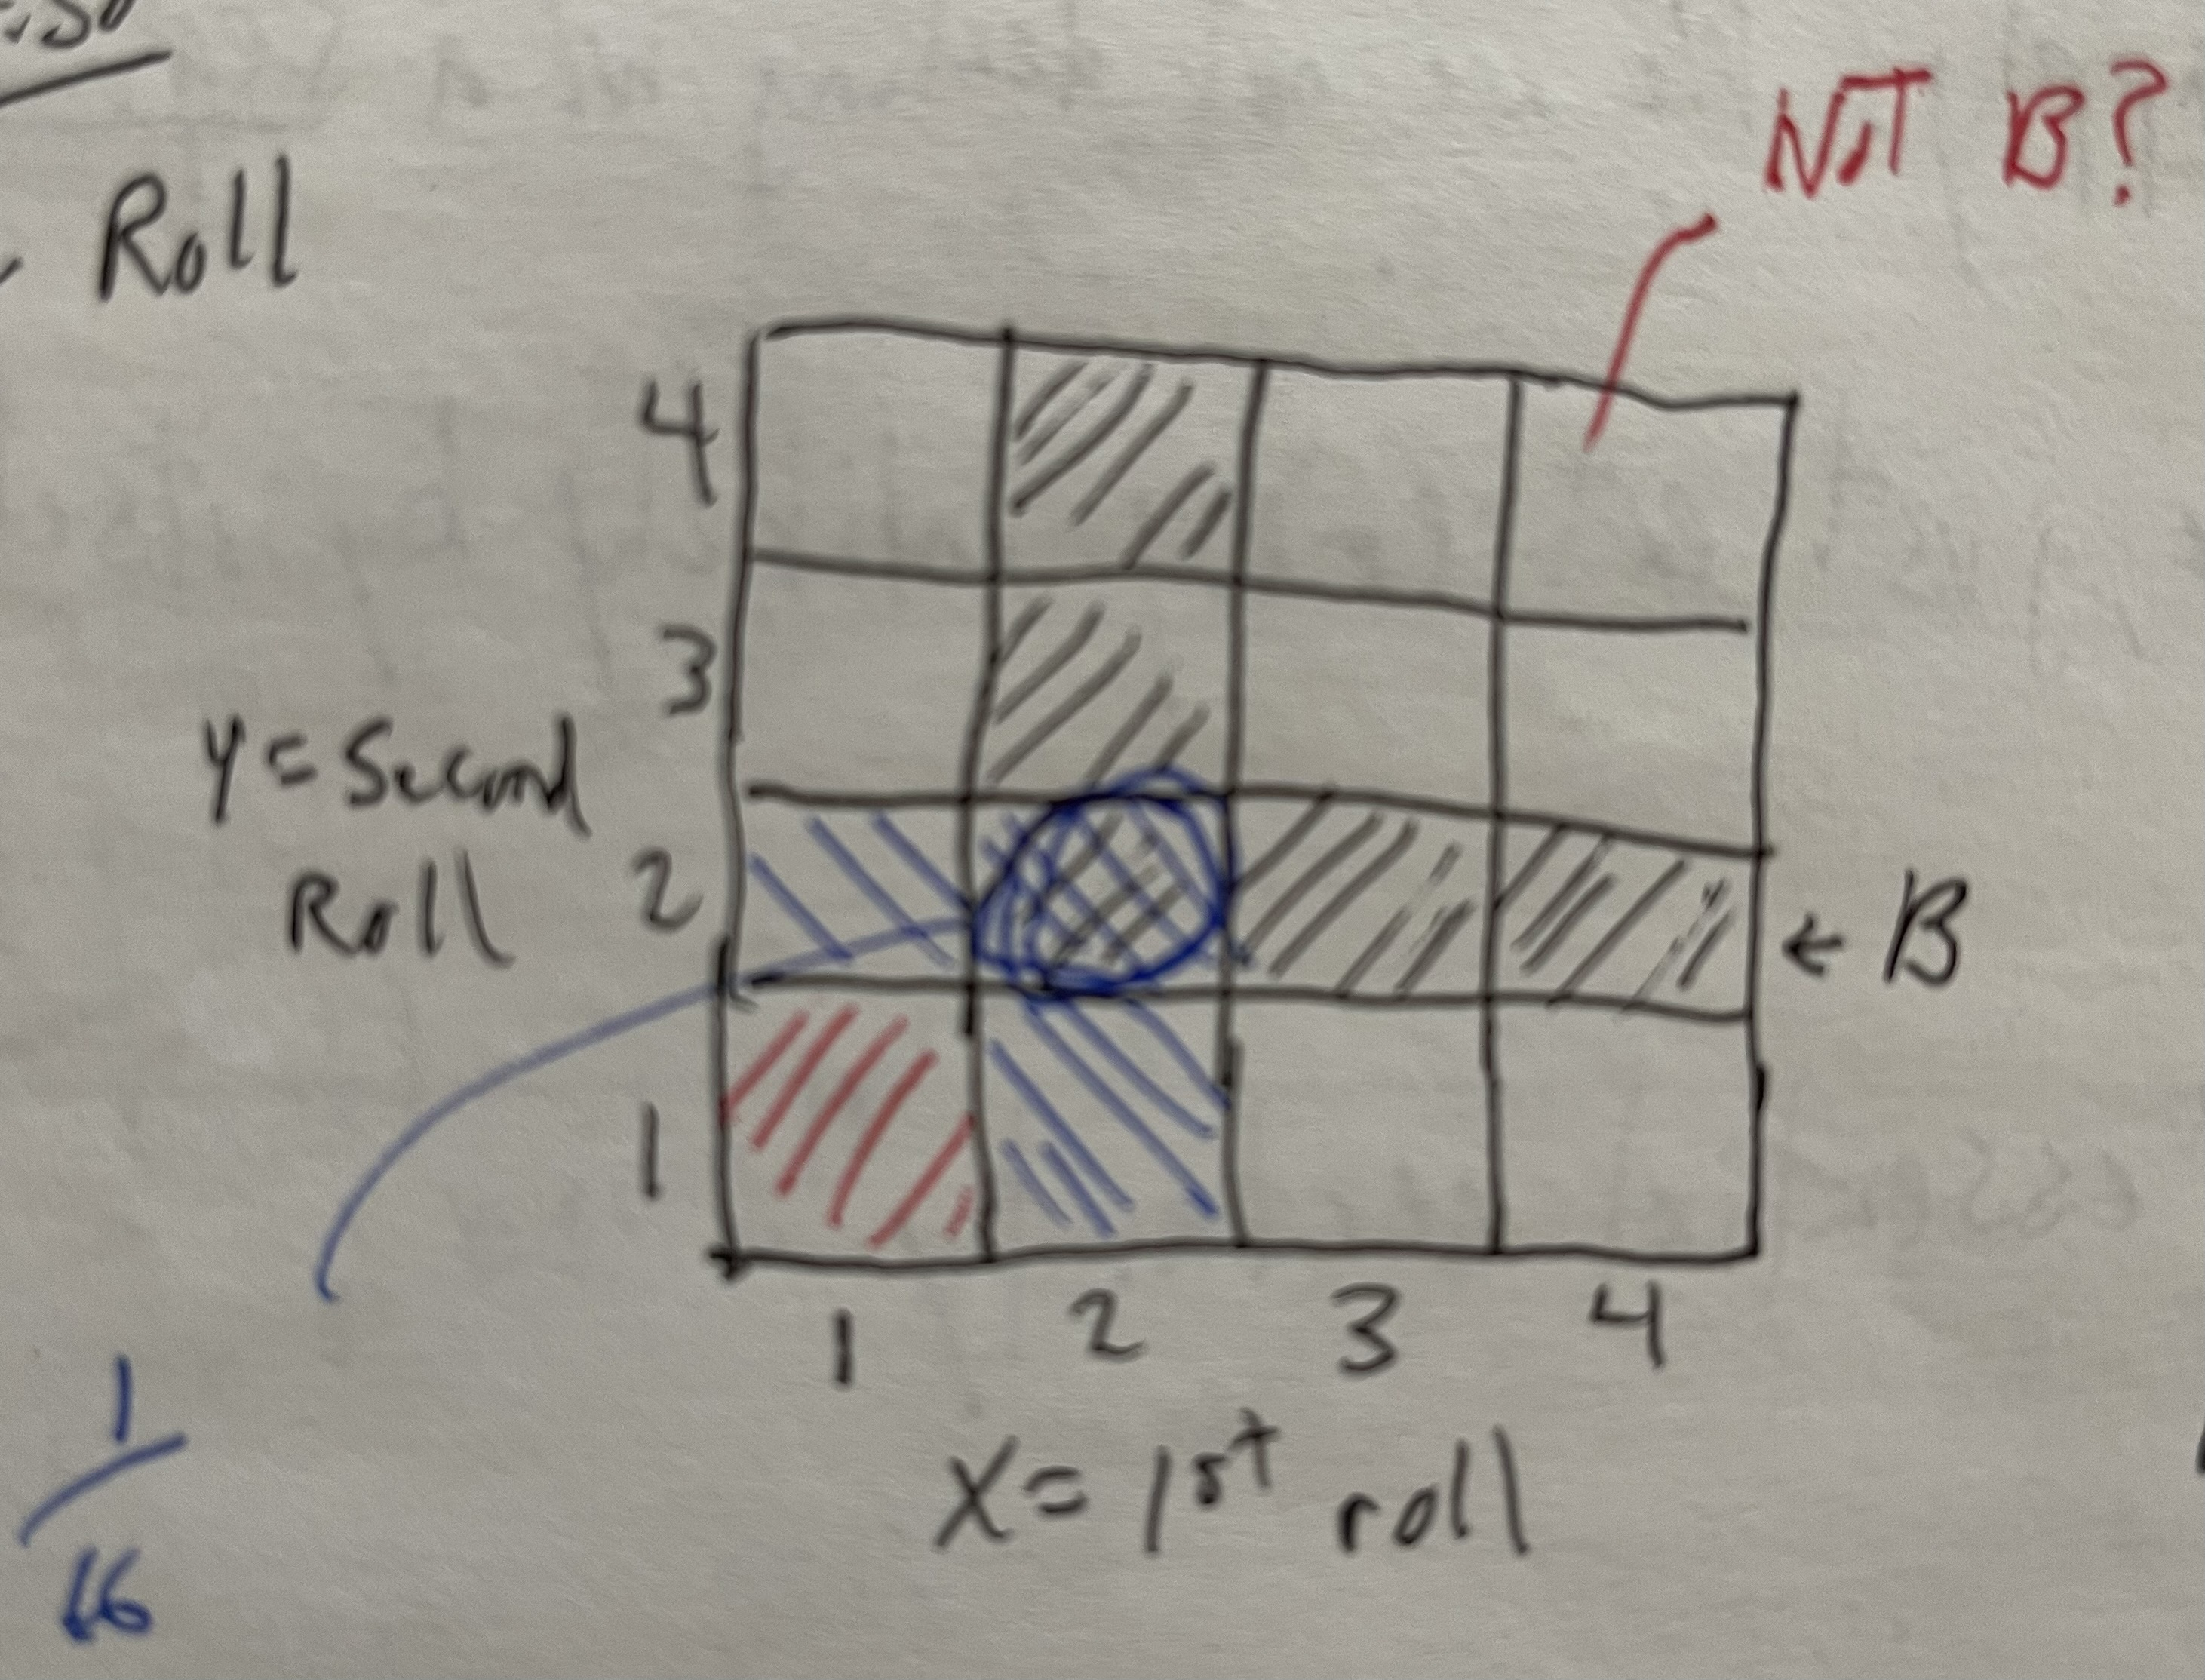
\includegraphics[width=6cm, height=4cm]{images/L02/dice_roll.jpeg}
\caption{Sample Space: Roll 2 Die}
\end{figure}

\subsection{Example: Airplane}

\marginpar{(24:45)}

\begin{itemize}
    \item Event A: Airplane is flying above
    \item Event B: Something registers on the radar screen
\end{itemize}

\begin{figure}[ht]
\centering
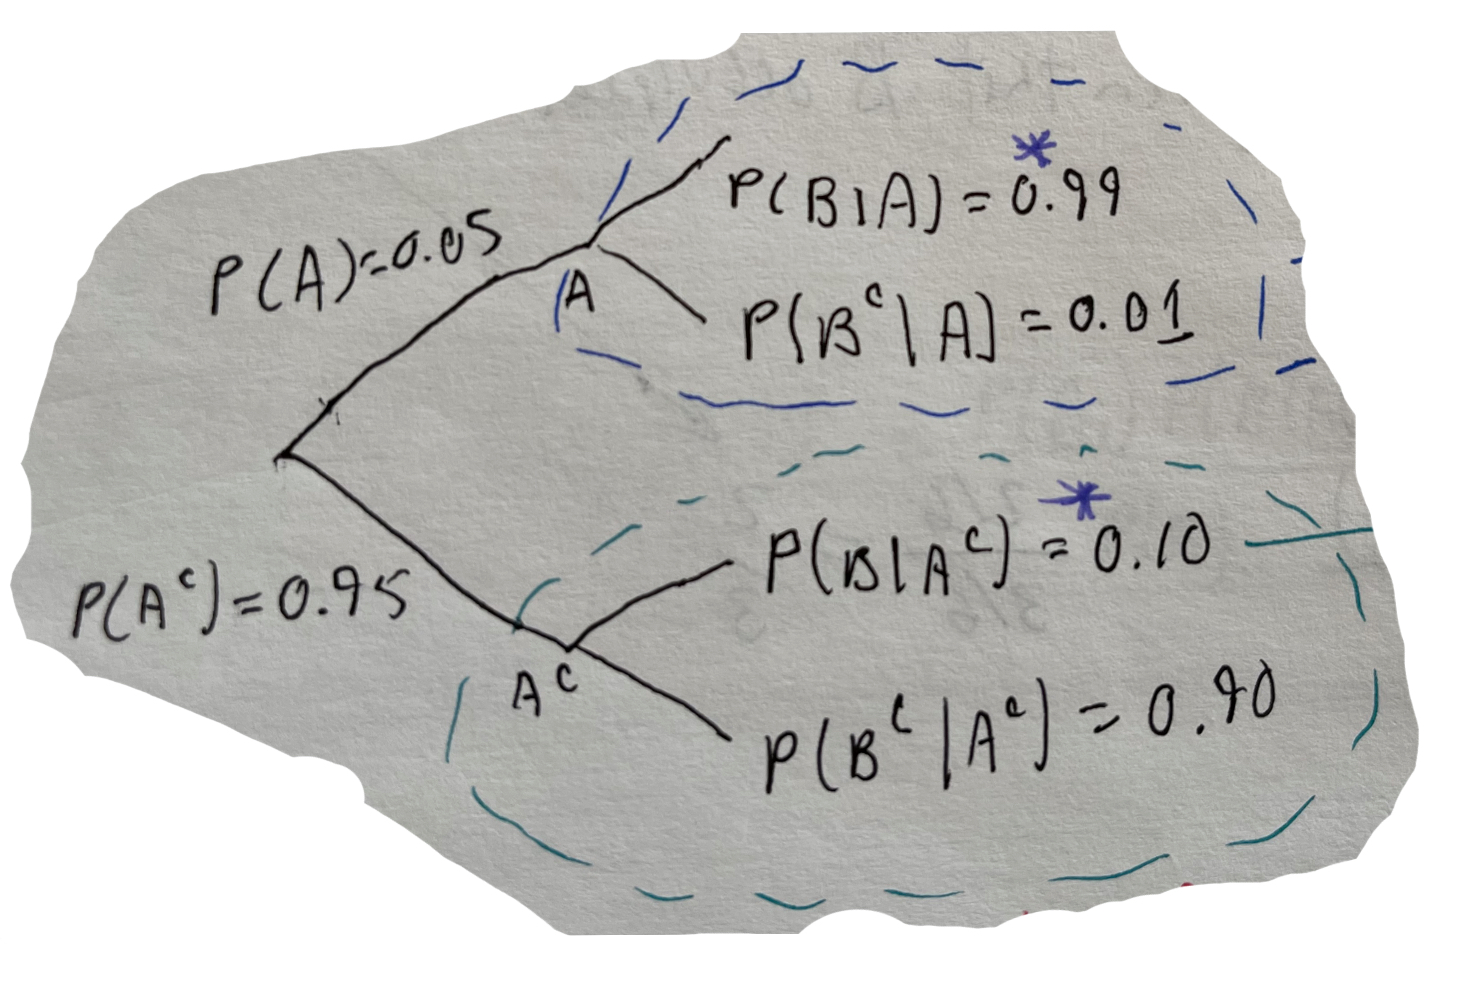
\includegraphics[width=5cm, height=4cm]{images/L02/airplane_radar.jpeg}
\caption{Airplane Probabilities}
\end{figure}

Can we derive ordinary probabilities starting from conditional?

\begin{align*}
P(A \cap B) = P(A)P(B|A) = 0.05\cdot 0.99 = 0.0495\\
P(B) =\\
P(A|B) =\\
\end{align*}

\marginpar{(28:25)}

What's the probability that our radar registers something? $P(B)$

\subsection{Multiplication Rule}

\marginpar{(34m)}

Multiply branches


\subsection{Total Probability Theorem}

Partition sample space.

\begin{figure}[ht]
\centering
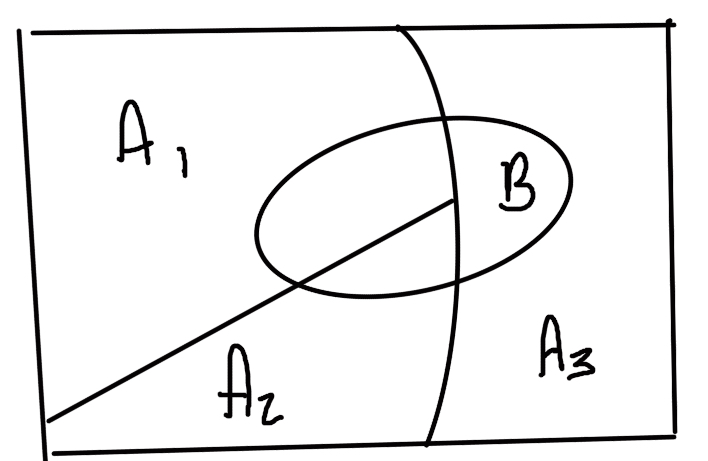
\includegraphics[width=5cm, height=4cm]{images/L02/total_prob.jpeg}
\caption{Total Probability}
\end{figure}

\begin{align*}
P(B)=P(A_1)P(B|A_1) + P(A_2)P(B|A_2) + P(A_3)P(B|A_3) = 1
\end{align*}

\subsection{Bayes Rule}

\begin{align*}
P(A_i|B) = \frac{P(A_i \cap B)}{P(B)} = \frac{P(A_i)P(B|A_i)}{P(B)} = \frac{P(A_i)P(B|A_i)}{\sum_j P(A_j)P(B|A_j)}
\end{align*}

$P(A_j)$ - prior probabilities

\section{Lecture 3: Independence}

\marginpar{\href{https://youtu.be/19Ql_Q3l0GA}{Video}}
\marginpar{\href{https://ocw.mit.edu/courses/6-041sc-probabilistic-systems-analysis-and-applied-probability-fall-2013/pages/unit-i/lecture-3/}{Lecture Home}}
\marginpar{\href{https://ocw.mit.edu/courses/6-041sc-probabilistic-systems-analysis-and-applied-probability-fall-2013/a2015627268f4846eb3b1368623ce46f_MIT6_041SCF13_L03.pdf}{Slides}}

Experiment

\begin{figure}[ht]
\centering
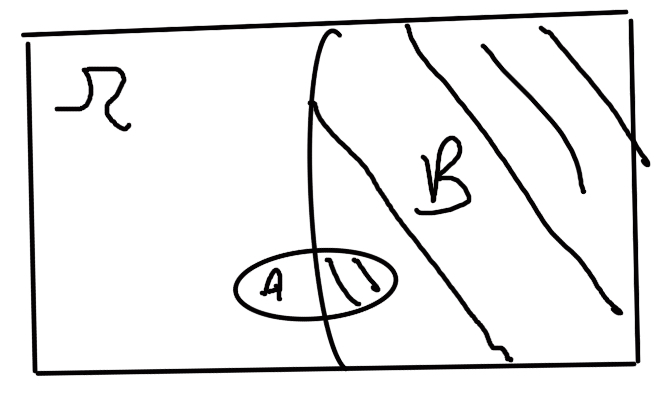
\includegraphics[width=5cm, height=4cm]{images/L03/independence.jpeg}
\caption{Independence}
\end{figure}

\begin{itemize}
    \item Outcome is in B so B is our new sample space
    \item Which A's were also assigned to B? $A \cap B$
\end{itemize}

New probabilities are conditional probabilities

\subsubsection*{Total Probability Theorem}

\begin{align*}
P(B)=P(A)P(B|A) + P(A^c)P(B|A^c)
\end{align*}

\marginpar{(4:25)} Trying to guess the state of the world based on your measurements.  That's what inference is all about.


Three Skills
\begin{itemize}
    \item Multiplication Rule - Follow tree along path
    \item Two
    \item Three
\end{itemize}

\subsection{Model Where We Toss a Coin 3 Times}

\begin{figure}[!ht]
\centering
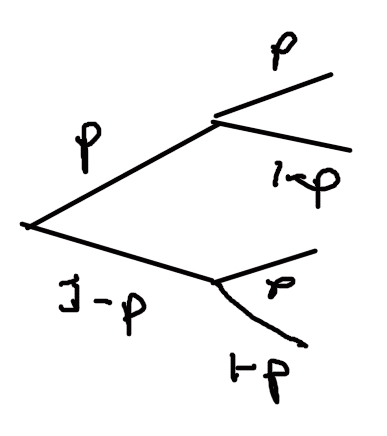
\includegraphics[width=5cm, height=4cm]{images/L03/coin_toss3.jpeg}
\caption{Coin Toss}
\end{figure}


\begin{align*}
P(H)=p, P(T)=1-p
\end{align*}

\begin{align*}
&P(THT)=(1-p)p(1-p)\\
&P(1\;Head)=3p(1-p)^2, \qquad \text{3 ways}\\
&P(\text{1st toss H}|1\;Head)=\frac{P(\text{1st toss H},1\;Head)}{P(1\;Head)}=\frac{P(HTT)}{P(1\;Head)}=\frac{p(1-p)^2}{3p(1-p)^2}=\frac{1}{3}
\end{align*}
% P(1\;Head)=3p(1-p)^2, \text{3 ways}\\
% 

\subsection{Independence}

\marginpar{(12m)}

First event gives no information for the second event.

Definition: $P(B|A)=P(B)$
$P(A \cap B)=P(A)P(B)$ This is a better definition.  It always works.
$P(A)=0 \Rightarrow independence$

\begin{figure}[ht]
\centering
\begin{tikzpicture}
\draw (0,0) rectangle (7,4);
\draw (2,2) ellipse (1cm and 1.2cm) node {A};
\draw (5,2) circle (1cm) node {B};
\end{tikzpicture}
\caption{Independent Events?} \label{fig:M22}
\end{figure}

% \begin{figure}[h]
% \centering
% \includegraphics[width=5cm, height=4cm]{IMG_1462.jpeg}
% \caption{Independent Events?}
% \end{figure}

No, separate has nothing to do with independence.  Information about A affects beliefs about B.

\subsubsection{Conditional Independence}

\marginpar{(22m)}

Definition of Conditional Independence:
\begin{align*}
P(A \cap B | C) = P(A|C)P(B|C)
\end{align*}

\marginpar{(24:00)} Independence and disjointness are two different things.

Physical link is choice of a coin.  Dependence.??

Bias coin example - see slide

\subsubsection{Independence of Collection of Events}

\marginpar{(31m)}

\begin{align*}
P(A_i \cap A_j \cap \cdots \cap A_q) = P(A_i)P(A_j)\cdots P(A_q)
\end{align*}

n=3
\begin{align*}
P(A_1 \cap A_2 \cap \cap A_3) = P(A_1)P(A_2)P(A_3)
\end{align*}

Pairwise Independence - Must apply to subcollection of events
\begin{align*}
P(A_1 \cap A_2 ) = P(A_1)P(A_2)\\
P(A_1 \cap A_3 ) = P(A_1)P(A_3)\\
P(A_2 \cap A_3 ) = P(A_2)P(A_3)\\
\end{align*}

\marginpar{(35m)} Independence and pairwise independence are two different things.

\subsubsection{Example: Pairwise but not Independent}

\begin{figure}[ht]
\centering
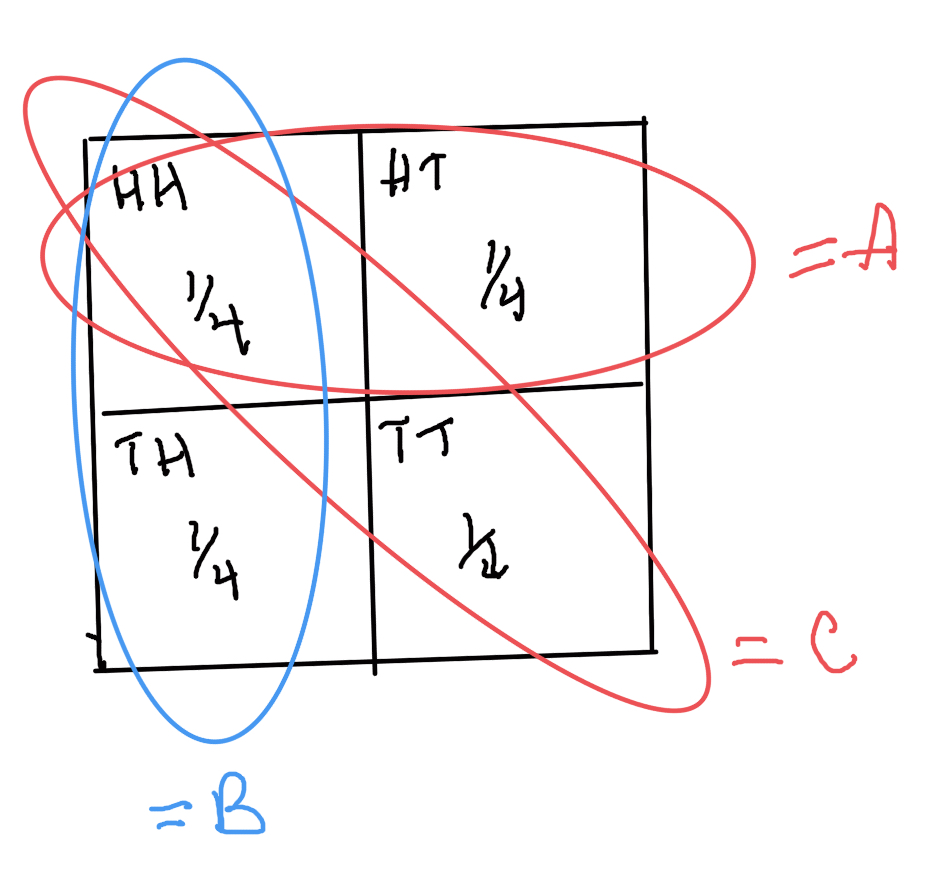
\includegraphics[width=5cm, height=4cm]{images/L03/collection_indep.jpeg}
\caption{...}
\end{figure}

They are independent mathematically:

\begin{align*}
P(A)=P(B)=\frac{1}{2}\\
\end{align*}

A={1st toss H}, B={2nd toss H}

C. First and second toss give same result

\begin{align*}
&P(C)=\frac{1}{2}\\
&P(C \cap A) = \frac{1}{4}\\
&P(A \cap B \cap C)x = \frac{1}{4}\\
&P(C|A \cap B) = 1, \qquad \text{No independence. Certain HH occurred}
\end{align*}

Therefore the three events are not independent but are pairwise independent.

\subsubsection{King's Sibling}

\marginpar{(41:25)}

\begin{figure}[ht]
\centering
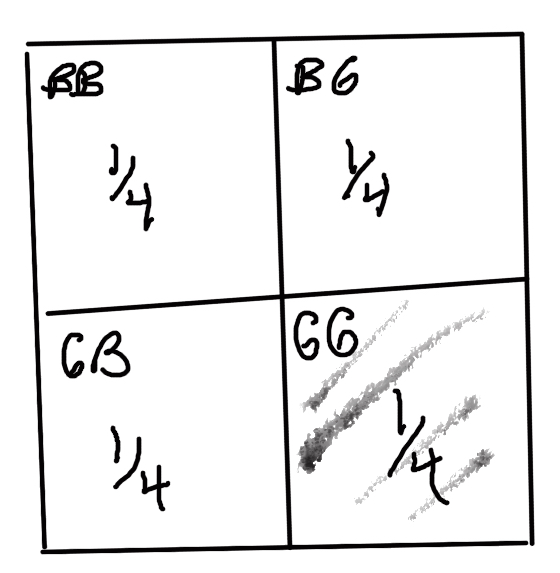
\includegraphics[width=5cm, height=4cm]{images/L03/kings_sibling.jpeg}
\caption{King's Sibling}
\end{figure}

In conditional probability $P(G)\frac{2}{3}$ (i.e. 2/3 of outcomes).

Hidden assumptions?  Things to consider: Maybe they had children until they had a boy $P(G)=1$

\section{Lecture 4: Counting}

\marginpar{\href{https://youtu.be/6oV3pKLgW2I}{Video}}

\begin{figure}[ht]
\centering
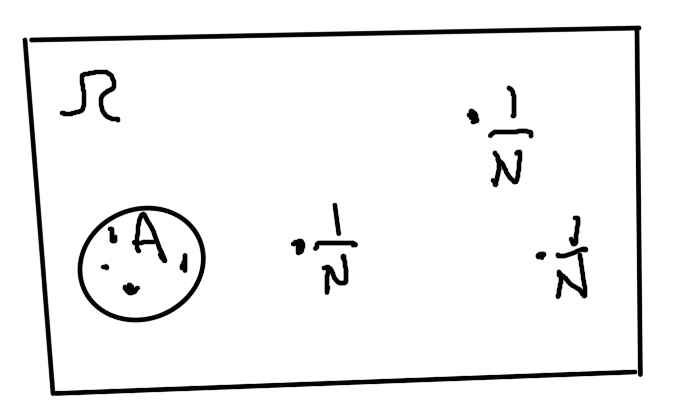
\includegraphics[width=5cm, height=4cm]{images/L04/counting.jpeg}
\caption{Counting}
\end{figure}

$\Omega=|N|$ - Need to determine N.
$|A|=n$

$$
P(A)=n\cdot \frac{1}{N}
$$

\marginpar{(3:30)} The most common trick is when considering a set, describe the outcomes through a sequential process.

\begin{figure}[ht]
\centering
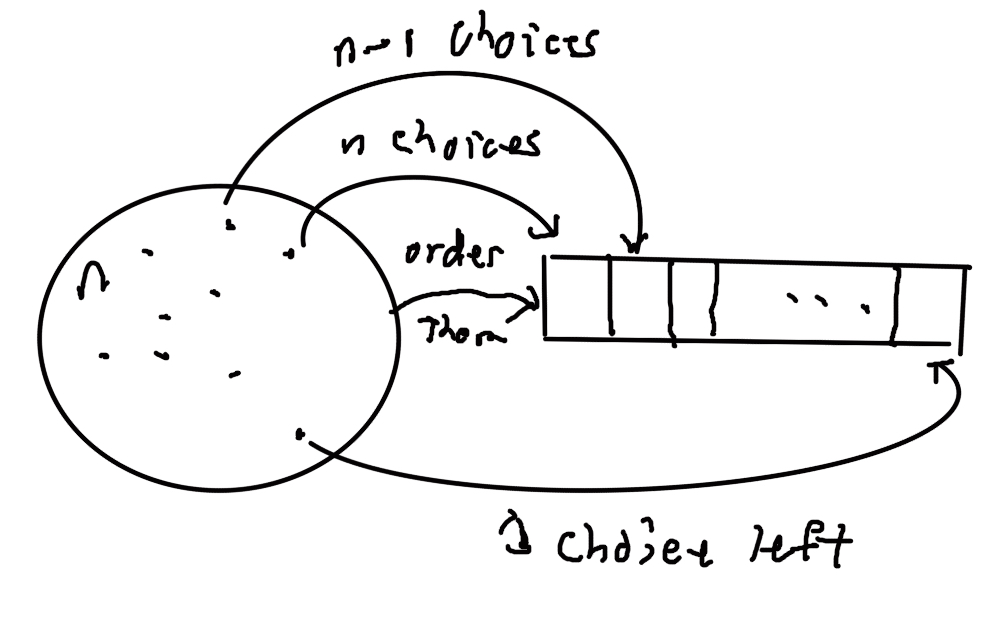
\includegraphics[width=5cm, height=4cm]{images/L04/seq_counting.jpeg}
\caption{Sequential Counting}
\end{figure}


Number of subsets of $\{1,,2, \ldots, n\}$.  For each element we have 2 choices: include/exclude.

\begin{align*}
    \underbrace{2\cdot 2\cdots 2}_{n} = 2^n
\end{align*}

\subsection{Example: Probability 6 rolls of 6-sided die are all different numbers}

\marginpar{(11:05)}

One outcome: $P(2,3,3,1,6,5)=P(2)P(3)P(3)P(1)P(6)P(5)=(\frac{1}{6})^6$

Number of elements in sample space: $\Omega=6^6$

\begin{align*}
\frac{|A|}{|\Omega|} = \frac{6!}{6^6}
\end{align*}

\marginpar{(16:30)}

Interested in subsets that have exactly k elements.

\begin{figure}[ht]
\centering
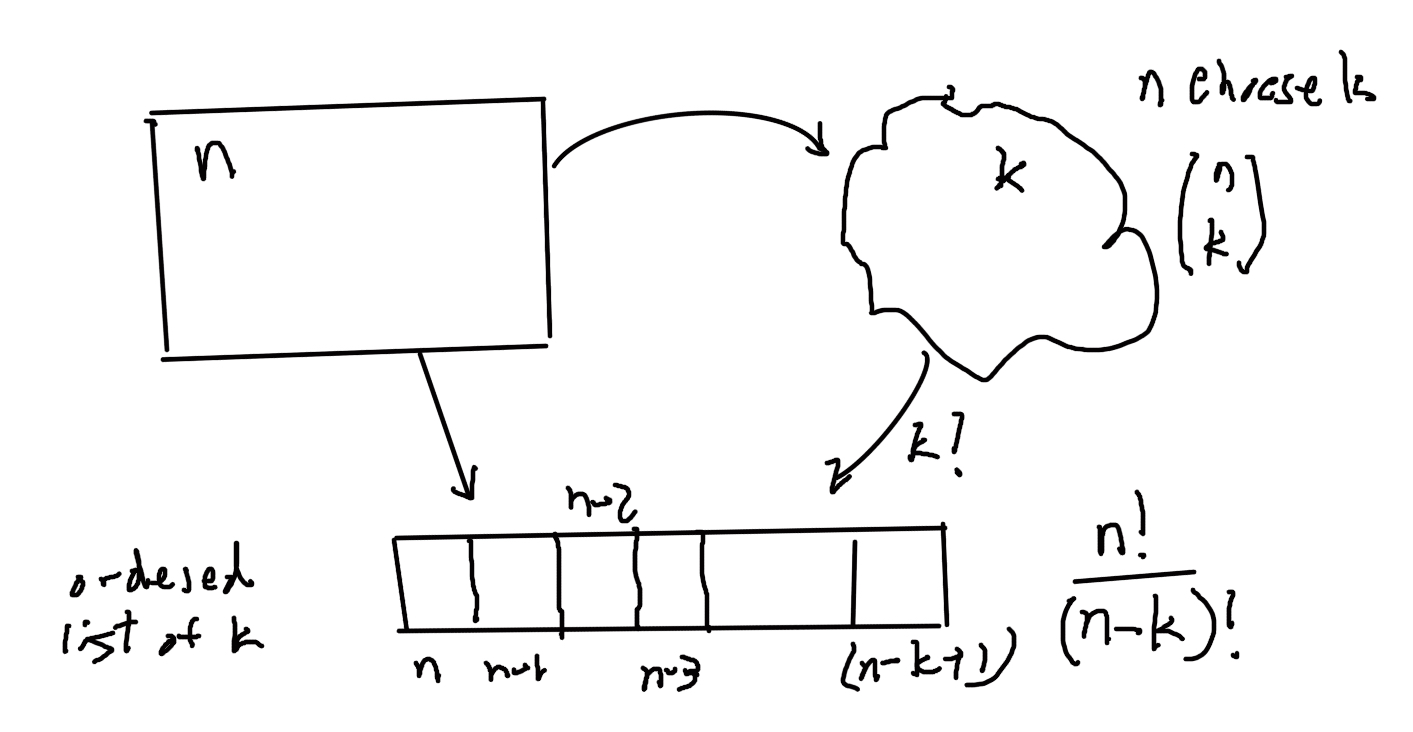
\includegraphics[width=5cm, height=4cm]{images/L04/sel_k_elems.jpeg}
\caption{Select k elements}
\end{figure}

e.g. N people in group and want to form k committees.

\begin{align*}
n(n-1)(n-2)\cdots (n-k+1)=\frac{n!}{(n-k)!} \quad choices
\end{align*}

\marginpar{(22:30)}

Hence:
\begin{align*}
{n \choose k}\cdot k! = \frac{n!}{(n-k)!} \Rightarrow {n \choose k} \frac{n!}{k!(n-k)!}
\end{align*}
This is the binomial coefficient.

\marginpar{(23:45)}

Defn: $0! = 1$

\begin{itemize}
    \item case k=n: $\frac{n!}{n!0!}=1$
    \item case k=0: $\frac{n!}{0!n!}=1$ 
\end{itemize}


\marginpar{(26m)}

$$\sum_{k=0}^n {n \choose k} = 2^n$$ \text{ we count the total number subsets}

\subsubsection{Binomial Probabilities}

\marginpar{(28:30)}

\begin{align*}
&P(H)=p\\
&P(HTTHHH)=p(1-p)(1-p)ppp = p^4(1-p)^2\\
&P(HHTTHH)= p^4(1-p)^2, \qquad \text{Same but different order}\\
&p^{\#heads}(1-p)^{\#tails}
\end{align*}

\marginpar{(32:25)}

\# k-head sequence = \# k-element subsets of ${n \choose k}$

\begin{figure}[h]
\centering
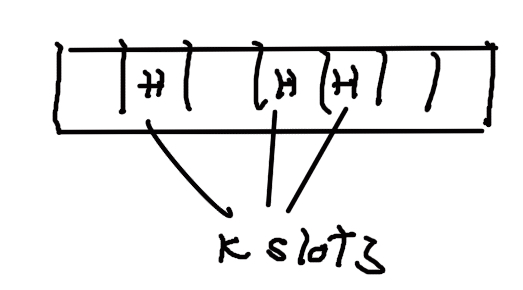
\includegraphics[width=5cm, height=4cm]{images/L04/k_slots.jpeg}
\caption{k slots}
\end{figure}

$$
\sum_{k=0}^{n} {n \choose k} p^k(1-p)^{n-k}=1
$$
$k=0,1,\ldots,n$ are binomial probabilities

\subsubsection{Coin Toss Experiment}

\begin{figure}[h]
\centering
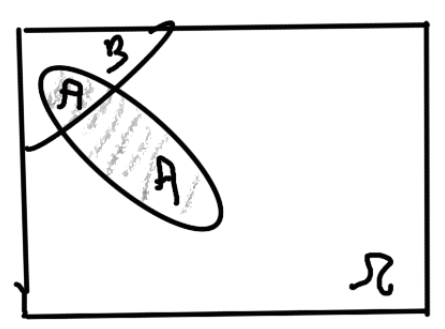
\includegraphics[width=5cm, height=4cm]{images/L04/coin_toss_exp.jpeg}
\caption{Coin Toss Experiment}
\end{figure}

Event B = \{3 out of 10 heads\}, Event A=\{first two tosses H\}

Events of $\Omega$ are not equally likely.

B: ${10 \choose 3}$, A: only third is uncertain: 8

\subsection{Partitions}

\marginpar{(42:55)}

\begin{figure}[h]
\centering
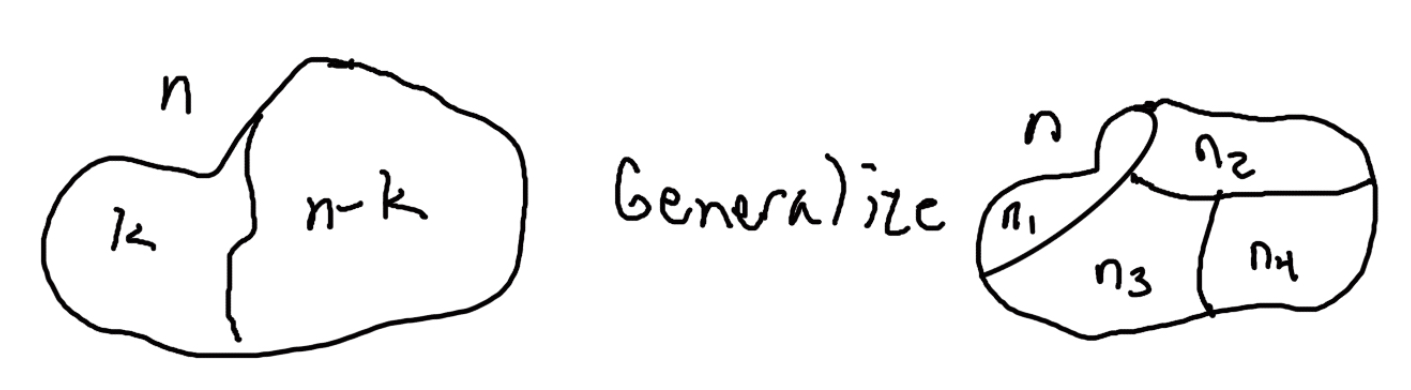
\includegraphics[width=8cm, height=4cm]{images/L04/generalize.jpeg}
\caption{Generalize}
\end{figure}

\begin{align*}
    {52 \choose 13}{39 \choose 13}{26 \choose 13}{13 \choose 13}
\end{align*}

\begin{align*}
    \frac{52!}{13!39!} \cdots = \frac{52!}{13!13!13!13!}
\end{align*}

\begin{align*}
    \frac{n!}{n_1!n_2!n_3!n_4!}
\end{align*}

$P(\text{each player gets ace}) = $ (see text book)

\subsection{Stars and Bars}


\section{Lecture 5: Discrete Random Variables; Probability Mass Functions; Expectations}

\marginpar{\href{https://youtu.be/3MOahpLxj6A}{Video}} Reading: 2.1-2.3 start 2.4

\begin{figure}[h]
\centering
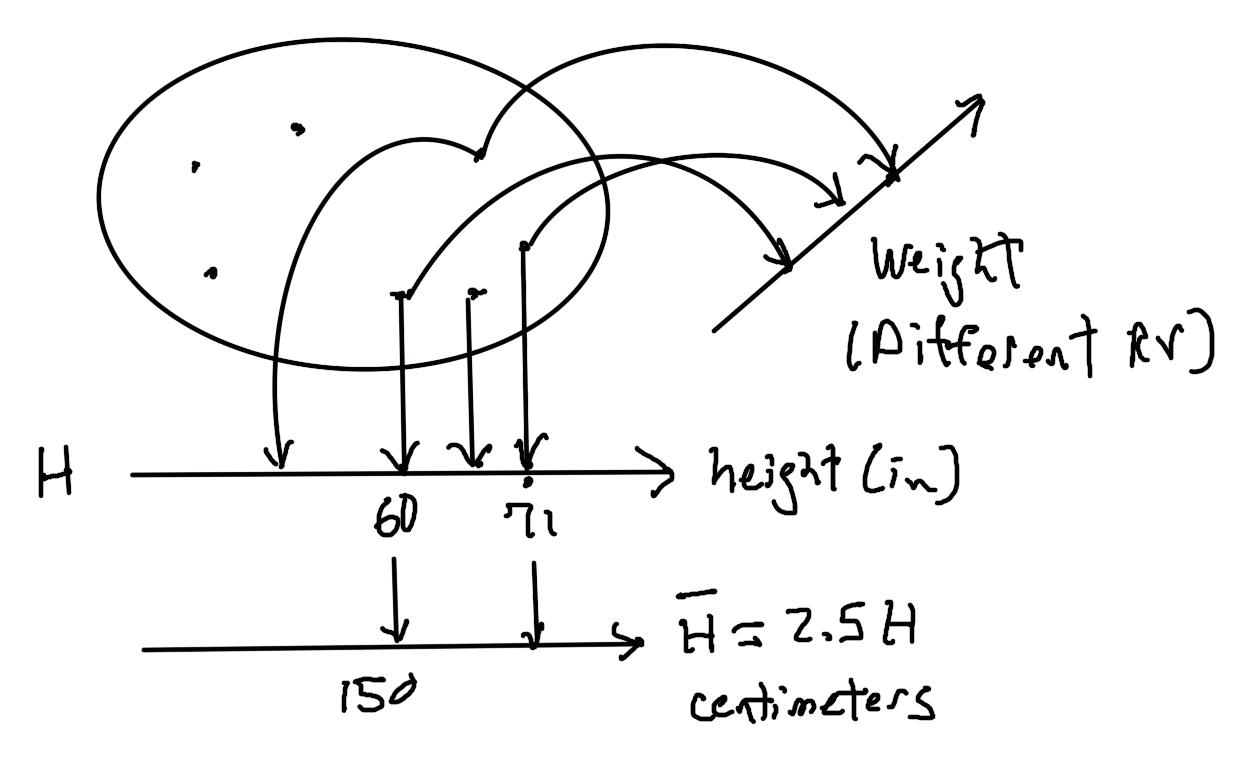
\includegraphics[width=5cm, height=4cm]{images/L05/diff_rvs.jpeg}
\caption{Experiment with Several RVs}
\end{figure}

\marginpar{(9:25)} Notation
\begin{itemize}
    \item Random variable X - function $\Omega \rightarrow \mathbb{R}$
    \item numerical value x - the amount of output of the function ($\in \mathbb{R})$
\end{itemize}

\subsection{PMF}

\marginpar{(11m)}

\begin{figure}[h]
\centering
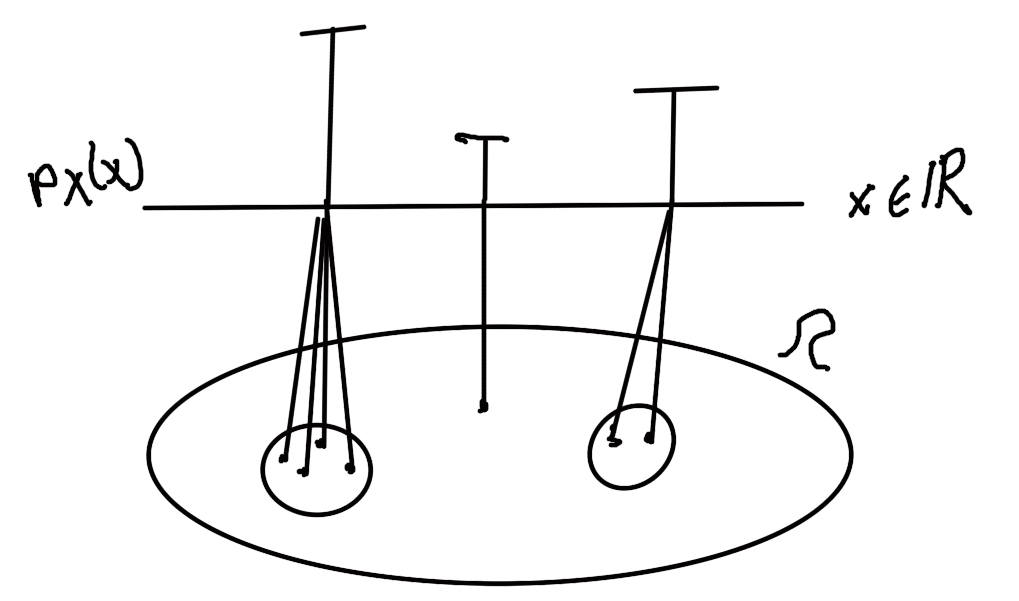
\includegraphics[width=5cm, height=4cm]{images/L05/pmf_px.jpeg}
\caption{Different RVs}
\end{figure}

\subsection{Example: \# tosses until get H (geometric RV)}

\begin{align*}
    p_X(x)=P(X=x)=P({\omega \in \Omega s.t. X(\omega)=x})
\end{align*}

\marginpar{(14:40)}

$$(1-p)^{k-1}p$$

```

\edef\mylst{"p","p(1-p)"}

\marginpar{(17m)}
\begin{figure}[h]
\centering
% 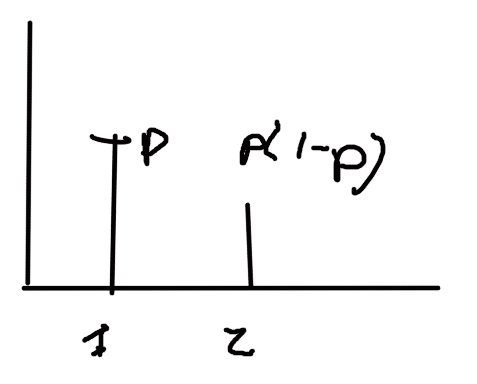
\includegraphics[width=5cm, height=4cm]{images/L05/geometric.jpeg}
\begin{tikzpicture}[scale = 0.7]
\begin{axis} [ymin = 0, ymax = 0.75, xmin = 0, xmax = 2.5,
        y tick label style={
        /pgf/number format/.cd,
            fixed,
            precision=2,
        /tikz/.cd,
        nodes near coords=\pgfmathsetmacro{\mystring}{{\mylst}[\coordindex]}\mystring,
    }]
\addplot+[ycomb] plot coordinates { (1, .5) (2, .3)}; 
\end{axis}
\end{tikzpicture}

\caption{Geometric PMF}
\end{figure}

\subsection{Example: Two independent rolls of fair tetrahedral die}

\marginpar{(18:50)}

\begin{figure}[h]
\centering
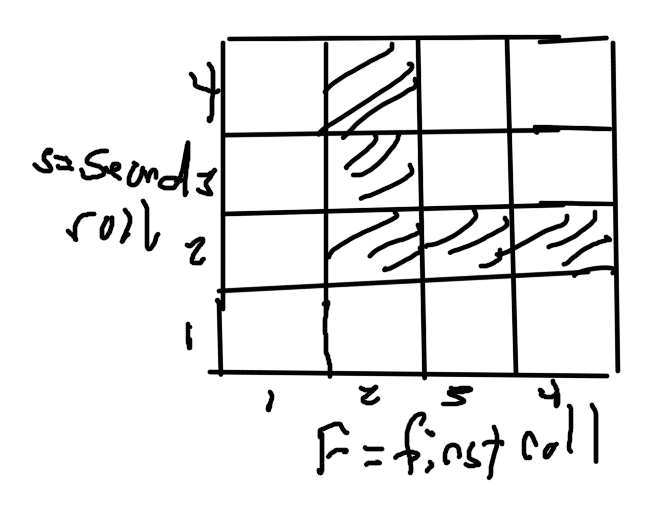
\includegraphics[width=5cm, height=4cm]{images/L05/min_2die_roll.jpeg}
\caption{Sample Space}
\end{figure}

\begin{itemize}
    \item F: outcome of first throw 2
    \item S: outcome of second throw 3
    \item X=min(F,S)
\end{itemize}

PMF: 
\begin{align*}
p_X(x)=5\frac{1}{16}=\frac{5}{16}
\end{align*}

\subsection{Binomial PMF}

\marginpar{(21m)}

X: number of heads in n fixed independent coin tosses

$P(H)=p$, let n=4

There are 6 events:
\begin{align*}
p_X(2)=P(HHTT) + P(HTHT) + \cdots + P(TTHH)\\
=6p^2(1-p)^2 \\
={4 \choose 2} p^2(1-p)^2 \\
\end{align*}

In general:

\begin{align*}
p_X(k)={n \choose k} p^k(1-p)n-k, \qquad k=0,\ldots,n\\
\end{align*}

\begin{align*}
p_X(k)=\binom{n}{k} p^k(1-p)n-k, \qquad k=0,\ldots,n\\
\end{align*}


\marginpar{(23:25)}
\begin{figure}[h]
\centering
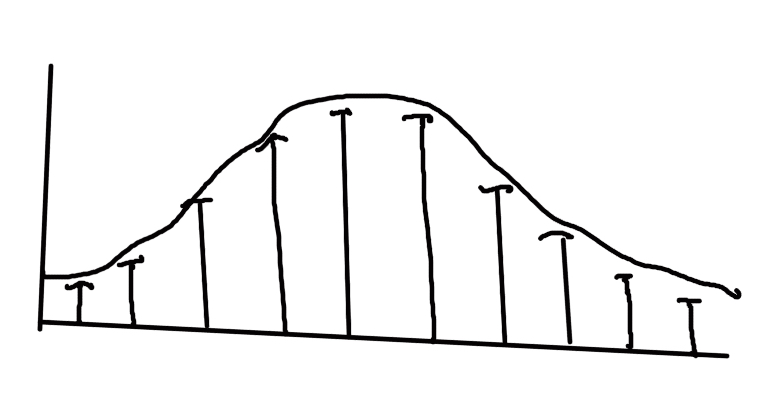
\includegraphics[width=5cm, height=4cm]{images/L05/bern_norm_approx.jpeg}
\caption{Large n gives bell curve}
\end{figure}

\subsection{Expected Value of a Random Variable}

\marginpar{(25:15)}

\begin{figure}[h]
\centering
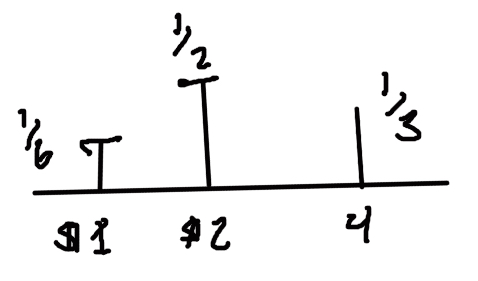
\includegraphics[width=5cm, height=4cm]{images/L05/EX_rv.jpeg}
\caption{PMF Payout}
\end{figure}

\begin{align*}
\frac{1}{6}\cdot 1 + \frac{1}{2}2 + \frac{1}{3}4 = 2.5, \qquad \text{avg payout}
\end{align*}

Expected value:
\begin{align*}
\sum_x p_X(x) \cdot x
\end{align*}
Note, this is also the center of gravity.

\subsection{Properties of Expectation}

\marginpar{(30:45)}

\begin{figure}[h]
\centering
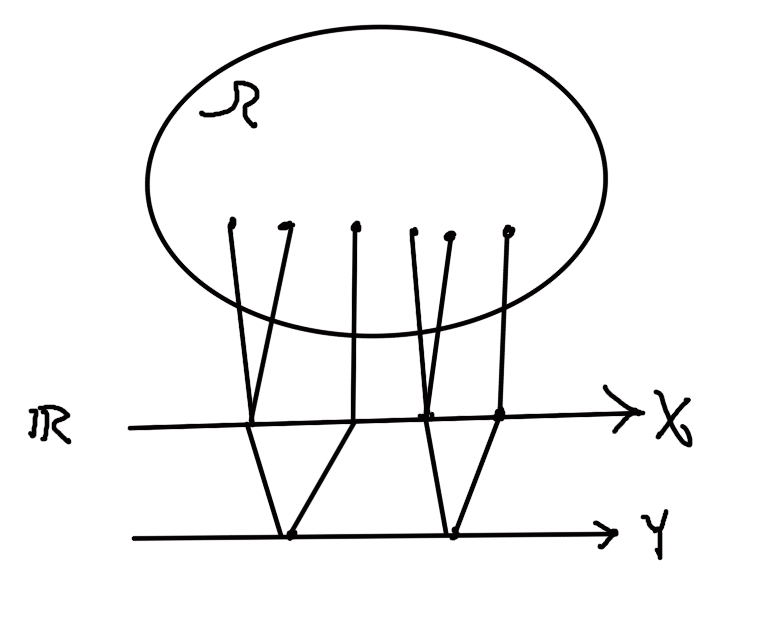
\includegraphics[width=5cm, height=4cm]{images/L05/EX_properties.jpeg}
\caption{Properties}
\end{figure}

\marginpar{(42:45)} In general, cannot reason on the average.  Only if $g(X)$ is linear.


\subsubsection{Properties}
$\alpha, \beta$ are constants

\begin{align*}
&E(\alpha] = \alpha\\
&E(\alpha X] = \alpha E[X]\\
&E[\alpha X + \beta] = \alpha E[X] + \beta
\end{align*}

\textbf{Proof: $E[\alpha X]= \alpha E[X]$}

MISSING

\subsection{Variance Properties}

\marginpar{(43m)}

\begin{align*}
var(\alpha X + \beta) = \alpha^2 var(X)
\end{align*}
Adding a constant has no affect to expectation.

\section{Lecture 6: Discrete Random Variable Examples; Joint PMFs}

\marginpar{\href{https://youtu.be/-qCEoqpwjf4}{Video}} Reading: 2.4-2.6

RV is a function from the sample space to the real numbers: $\Omega \rightarrow \mathbb{R}$

\marginpar{(8m)}

\begin{align*}
E[X-E[X]] = E[X] - E[X] = 0
\end{align*}

If we want to say something about how far we are from the mean, could take $|abs|$.

\begin{align*}
var(X)=E[(X-E[X])^2] = \sum_x(x - E[X])^2 p_X(x)\\
= E[X^2] -(E[X])^2
\end{align*}

std = $\sigma_X = \sqrt{var(X)}$

\subsection{Random Speed}

\marginpar{(12m)}

Traverse 200 mile distance at constant but random speed v.


\begin{figure}[h]
\begin{tikzpicture}
\centering
\begin{axis}[
    % axis lines = left,
   xtick={1,200},
    ytick={.5,.5},
]
\addplot+[ycomb] plot coordinates
    {(1,.5) (200,.5) };
\end{axis}
\end{tikzpicture}
\caption{$p_V(v)$}
\end{figure}

$d=200$, $T=t(v)-200/v$

\begin{align*}
E[V] = \frac{1}{2}1 + \frac{1}{2}200 = 100.5
\end{align*}

\begin{align*}
var[V] = \frac{1}{2}(1-100.5)^2 + \frac{1}{2}(200 -100.5)^2 = 100^2
\end{align*}

$\sigma_V = \sqrt{100^2}=100$

\marginpar{(14:15)}

Random variable T: time in hours=T=$T(v)=$

\begin{align*}
E[T] = E[t(v)] = \sum_v t(v)p_V(v) = \frac{1}{2}200 + \frac{1}{2}2 = 100.5
\end{align*}

\begin{align*}
E[TV] = 200 \ne E[T]E[V]
\end{align*}

\begin{align*}
E[200/V] = E[T] \ne 200/E[V] \approx 2
\end{align*}

\subsection{Conditional PMF and Expectation}

\marginpar{(18m)}

\begin{align*}
p_{X|A}(x) = P(X=x|A)\\
E[X|A] = \sum_x x p_{X|A}(A) ???check
\end{align*}

Let $A=(X \ge 2)$

\begin{align*}
p_{X|A}(x) = \frac{1}{3},\; x=2,3,4
\end{align*}

Conditional PMF's need to add to 1.

\begin{align*}
E[X|A] = \frac{1}{3}2 + \frac{1}{3}3 + \frac{1}{3}4=3
\end{align*}


\begin{figure}[h]
\centering
\begin{tikzpicture}
\begin{axis}[
    % axis lines = left,
   xtick={1,2,3,4},
    ytick={0,.25,1},
]
\addplot+[ycomb] plot coordinates
    % {(0,.25) (1,.25) (2,.25) (3,.25) (4,.25)};
    {(1,.25) (2,.25) (3,.25) (4,.25)};
\end{axis}
\end{tikzpicture}
\caption{$p_X(x)$}
\end{figure}

\marginpar{(23:25)}

\subsection{Geometric PMF}
\marginpar{(24:50)}

\subsection{Total Expectation Theorem}

\marginpar{(34:30)}

Partition sample space into disjoint events $A_1, \ldots, A_n$

Divide and Conquer method.

\begin{figure}[h]
\centering
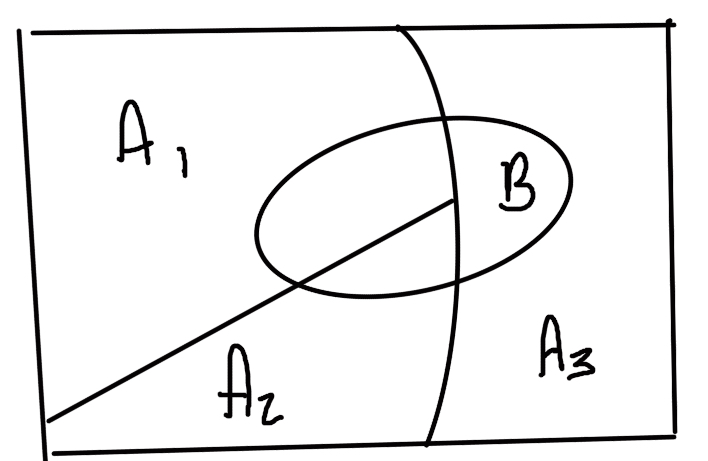
\includegraphics[width=5cm, height=4cm]{images/L02/total_prob.jpeg}
\caption{Total Probability}
\end{figure}

\begin{align*}
P(B)=P(A_1)P(B|A_1) + \cdots + P(A_n)P(B|A_n) - \text{Total Probability Theorem} \\
?? p_X(x) = P(A_1)p_{X|A_1}(x) + \cdots + P(A_n)p_{X|A_n}(x) - \text{Translated with PMF's}\\
\end{align*}

\begin{align*}
E[X]=P(A_1)E(X \mid A_1) + \cdots + P(A_n)E(X \mid A_n)
\end{align*}

\subsection{Divide and Conquer with Geometric Variable}

\marginpar{(37:25)}

$A_1:\{X=1\}, A_2:\{X >1\}$

\begin{align*}
E[X]=P(X=1)E(X|X=1) + P(X > 1)E(X \mid X>1)
\end{align*}
Solve to get $E[X]=\frac{1}{p}$

\begin{align*}
E[X|X-1 >0] = E[X-1 \mid X-1>0] + 1 ??
\end{align*}

\subsection{Joint PMFs}

\marginpar{(48:30)} Joint probabilities

\begin{figure}[h]
\centering
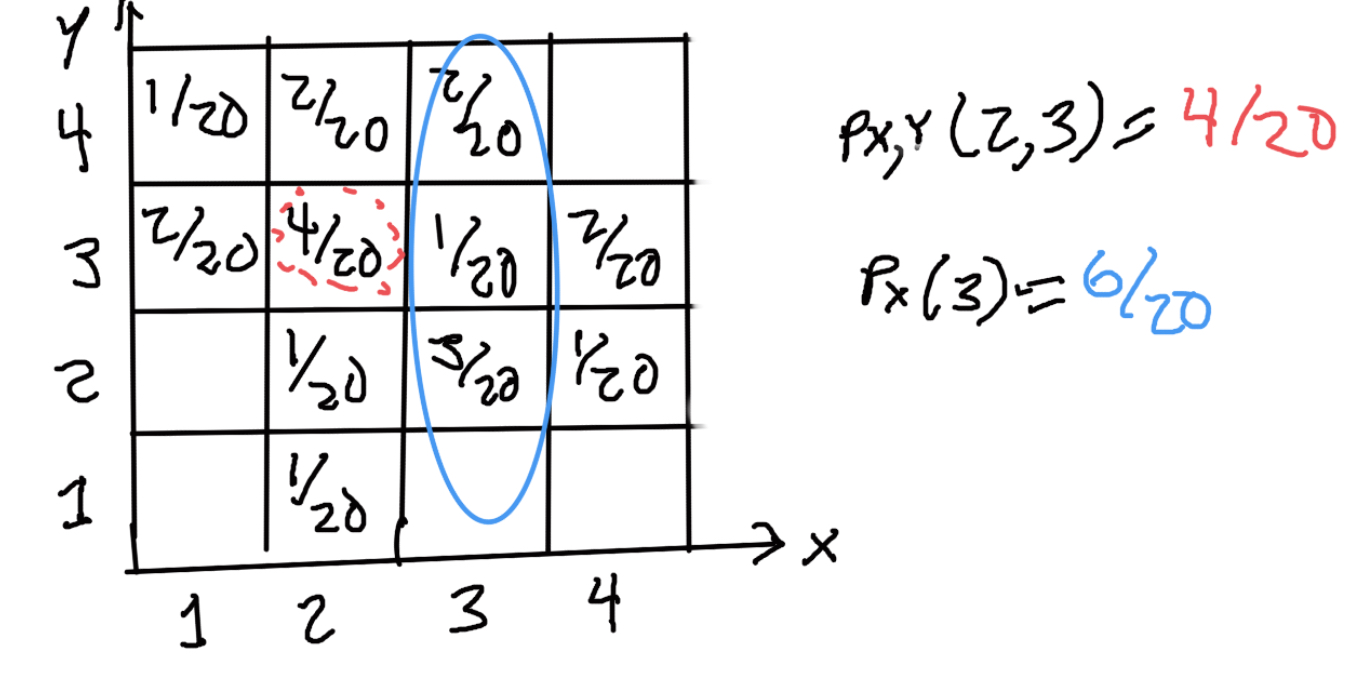
\includegraphics[width=8cm, height=4cm]{images/L06/joint_pmf.jpeg}
\caption{Joint PMFs}
\end{figure}

\section{Lecture 7: Multiple Discrete Random Variables}

\marginpar{\href{https://youtu.be/EObHWIEKGjA}{Video}} Reading: Finish Chapter 2

\subsection{Independent Random Events}

\marginpar{(8m)}

\begin{align*}
p_{X,Y,Z}(x,y,z)=p_X(x)p_{Y|X}(y|x)p_{Z|X,Y}(z|x,y)
\end{align*}

Random variables X,Y,Z are independent if:
\begin{align*}
p_{X,Y,Z}(x,y,z)=p_X(x)p_{Y}(y)p_{Z}(z)
\end{align*}

\begin{figure}[h]
\centering
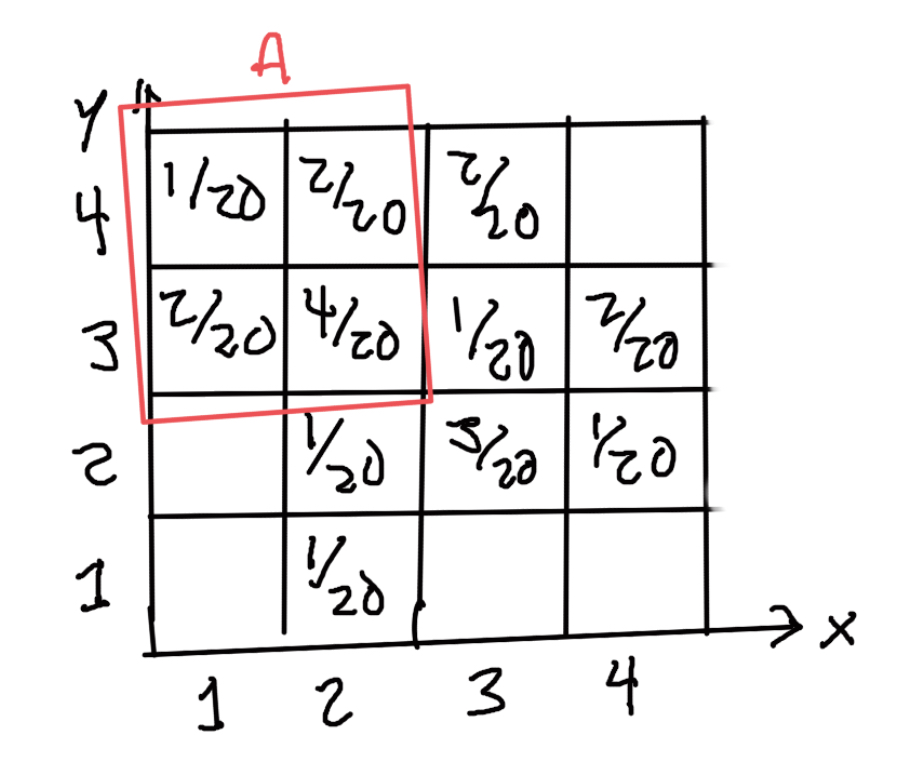
\includegraphics[width=6cm, height=4cm]{images/L07/IMG_1544.jpeg}
\caption{Joint PMFs}
\end{figure}

\begin{figure}[h]
\centering
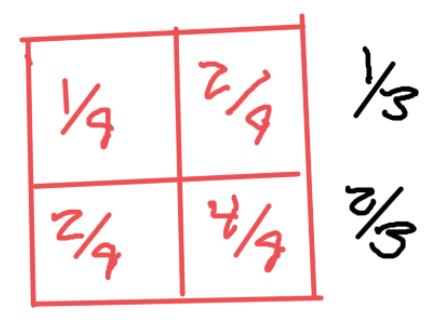
\includegraphics[width=5cm, height=4cm]{images/L07/IMG_1545.jpeg}
\caption{Joint PMFs}
\end{figure}

\marginpar{(19m)}

\marginpar{(28m)}

\subsection{Binomial Mean and Variance}
\marginpar{(32m)}

\subsection{Hat Problem}

\marginpar{(39m)}

\begin{figure}[h]
\centering
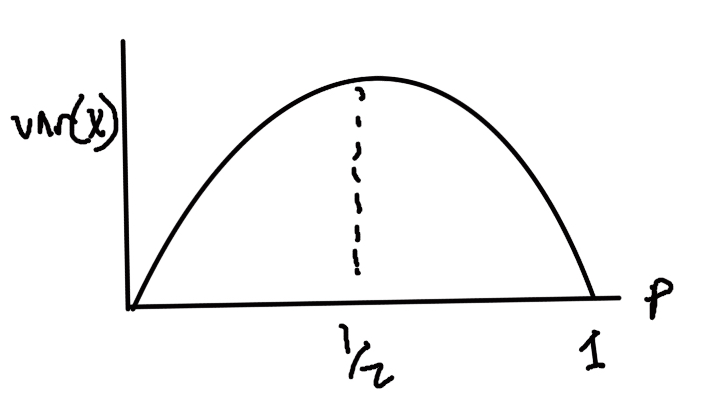
\includegraphics[width=5cm, height=4cm]{images/L07/bin_hat_problem.jpeg}
\caption{Hat Problem}
\end{figure}

\marginpar{(43:20)}

\begin{align*}
var(X) = E[X^2] - (E[X])^2
\end{align*}

$E[X^2]=2$

$var(X)=2-1=1$

\section{Lecture 8: Continuous Random Variables}

\marginpar{\href{https://youtu.be/mHfn_7ym6to}{Video}}

Read: 3.1-3.3

\subsection{Continuous Random Variables and PDF's}

Random variables are functions on the sample space.

\begin{figure}[!ht]
\centering
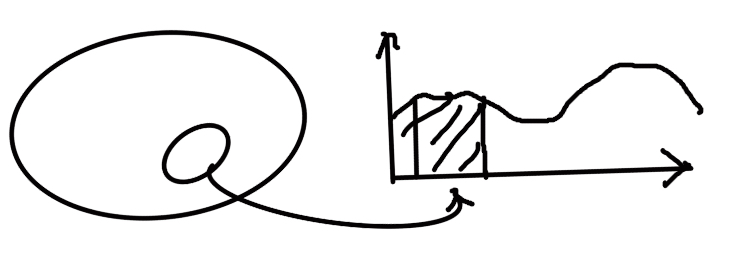
\includegraphics[width=6cm, height=4cm]{images/L08/continuous_rv.jpeg}
\caption{x}
\end{figure}

\begin{align*}
P(a \le X \le b) = \int_a^b f_X(x)dx \\
\int_{-\infty}^\infty f_X(x)dx=1 \\
P(X=a)=0 \\
f_X \ge 0\\
\end{align*}

\subsection{Mean and Variance}

\marginpar{(13:55)}

\begin{align*}
E[X] = \int_{-\infty}^{\infty} x f_X(x)dx
\end{align*}

\begin{align*}
E[g(X)] = \int_{-\infty}^{\infty} g(x) f_X(x)dx
\end{align*}

\begin{align*}
var[X] = \sigma_X^2 = \int_{-\infty}^{\infty} (x - E[X]^2 f_X(x)dx = E[X^2] - (E[X])^2
\end{align*}

\subsection{Continuous Uniform Random Variable}

\marginpar{(13:55)}

\begin{center}
    \begin{tikzpicture}[scale = 0.6]
       \begin{axis}[unit vector ratio=1 1.65 1,
       axis lines = left,
       ymin=-0.0025,ymax=1.2075,xmin=-0.5, xmax = 2.2, 
       % xtick={0,0.5,1,1.5,2,2.5,3},ytick={0.5,1}
       xticklabels={,,},yticklabels={,,}
       ]
       \addplot[very thick,domain=-1:0,blue] {0};
       \addplot[very thick,domain=0:1,blue] {0.5};
       \addplot[very thick,domain=1:2,blue] {0};
       % \addplot[very thick,domain=2:2.5,blue] {1};
       % \addplot[very thick,domain=2.5:3.3,blue] {0};
       \draw[very thick, blue, -] (axis cs:0,0) -- (axis cs:0,0.5);
       \draw[very thick, blue, -] (axis cs:1,0) -- (axis cs:1,0.5);
       % \draw[very thick, blue, -] (axis cs:2,0) -- (axis cs:2,1);
       % \draw[very thick, blue, -] (axis cs:2.5,0) -- (axis cs:2.5,1);
    \end{axis}
\end{tikzpicture}
\end{center}

\begin{figure}[h]
\centering
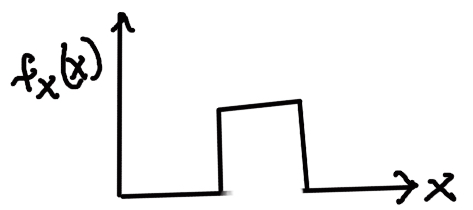
\includegraphics[width=6cm, height=4cm]{images/L08/continuous_unif_pdf.jpeg}
\caption{Continous Uniform Random Variable}
\end{figure}

$h=\frac{1}{b-a}$

Intervals of the same length have the same probability.

\begin{align*}
f_X(x)=\begin{cases}\frac{1}{b-a}, a \le x \le b\\
        0, otherwise
        \end{cases}
\end{align*}

\begin{align*}
E[X] = \int_a^b x\cdot \frac{1}{b-a}dx = \frac{a+b}{2}, \text{midpoint}
\end{align*}

\begin{align*}
\sigma_X^2= = \int_a^b (x - \frac{a+b}{2})^2 = \frac{1}{b-a}dx = \frac{(b-a)^2}{12}\\
\sigma_x = \frac{b-a}{\sqrt{12}}
\end{align*}

\subsection{Cumulative Distribution Function (CDF)}

\marginpar{(20:35)}

Unifying concept of continuous and discrete random variables.

\begin{align*}
F_X(x) = P(X \le x) = \inf_{-\infty}^{\infty} f_X(t)dt
\end{align*}

\begin{figure}[ht]
\centering
\begin{minipage}{.45\linewidth}
  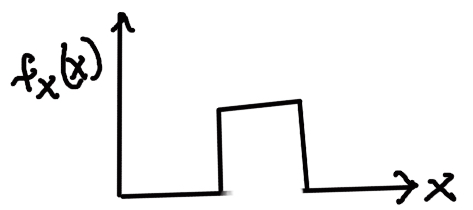
\includegraphics[width=\linewidth]{images/L08/continuous_unif_pdf.jpeg}
  \caption{PMF}
  \label{continuous_unif_pdf}
\end{minipage}
\hspace{.05\linewidth}
\begin{minipage}{.45\linewidth}
  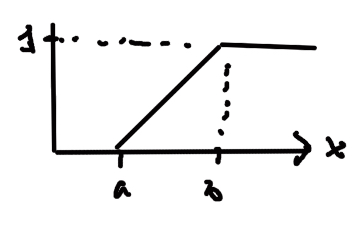
\includegraphics[width=\linewidth]{images/L08/continuous_cdf.jpeg}
  \caption{CDF}
  \label{continuous_cdf}
\end{minipage}
\end{figure}

\edef\mylst{"1/6","3/6","2/6",""}

\begin{figure}[ht]
\centering
\begin{minipage}{.45\linewidth}
  % 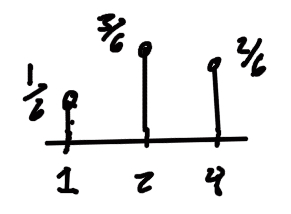
\includegraphics[width=\linewidth]{images/L08/discrete_pmf.jpeg}
\begin{tikzpicture}[scale = 0.7]
\begin{axis} [ymin = 0, ymax = 0.75, xmin = 0, xmax = 4.5,
		y tick label style={
        /pgf/number format/.cd,
            fixed,
            precision=2,
        /tikz/.cd,
        % nodes near coords = {1/6 3/6}
        % nodes near coords
        nodes near coords=\pgfmathsetmacro{\mystring}{{\mylst}[\coordindex]}\mystring,
    }]
\addplot+[ycomb] plot coordinates { (1, 1/6) (2, 3/6) (4, 2/6)}; 
\end{axis}
\end{tikzpicture}
  
  \caption{PMF}
  \label{img1}
\end{minipage}
\hspace{.05\linewidth}
\begin{minipage}{.45\linewidth}
  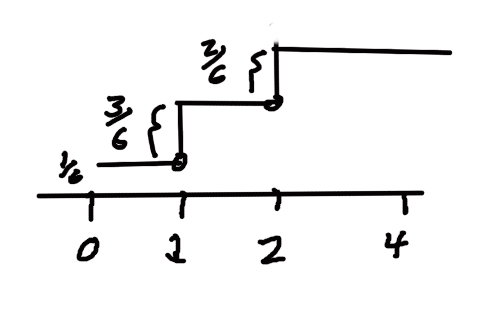
\includegraphics[width=\linewidth]{images/L08/discrete_cdf.jpeg}
  \caption{CDF}
  \label{img2}
\end{minipage}
\end{figure}

\marginpar{(27:40)}

Not all RV's are continuous or discrete.  Can be neither or a mixture of both.

\begin{figure}[h]
\centering
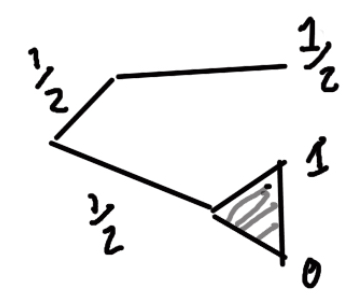
\includegraphics[width=5cm, height=4cm]{images/L08/mixed_rv.jpeg}
\caption{Mixed RV/Mixed Distribution}
\end{figure}

\subsection{Gaussian (Normal) PDF}

\marginpar{(27:40)}

Sum of many small RVs is Normal.

\begin{figure}[h]
\centering
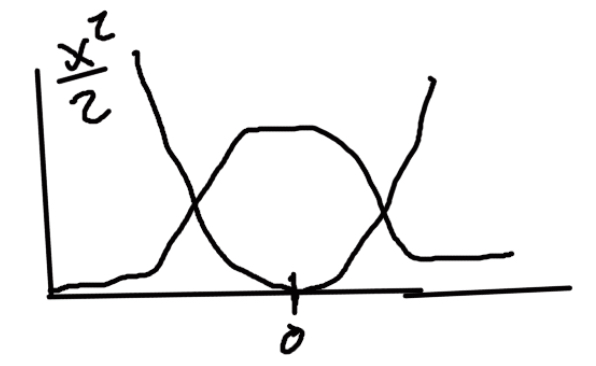
\includegraphics[width=5cm, height=4cm]{images/L08/gaussian_pdf.jpeg}
\caption{x}
\end{figure}

Standard normal $N(0,1)$

\begin{align*}
f_X(x) = \frac{1}{\sqrt{2\pi}} e^{-x/2}
\end{align*}

$\frac{1}{\sqrt{2\pi}}$ is the constant that makes the integral integrate to 1.

Gaussian centered at different places
\begin{align*}
&f_X(x) = \frac{1}{\sigma\sqrt{2\pi}} e^{-(x-\mu)/2\sigma^2}\\
&\mathbb{E}[X]=\mu \\
&var(X)= \sigma^2
\end{align*}

Let $Y=aX+b$
\begin{align*}
&E[Y]=a\mu+b\\
&var(Y)= a^2 \sigma^2\\
&Y \sim N(a\mu+b, a^2 \sigma^2)\\
\end{align*}

\marginpar{(41:30)}

\begin{align*}
\int_{-\infty}^{\bar{x}} e^{-x^2/2}dx
\end{align*}

No closed form solution.  We tabulate it.  There's only a table for standard normal $N(0,1)$.

If $X \sim N(2,16)$:

\begin{align*}
P(X \le 3) = P\left( \frac{X-2}{4} \le \frac{3-2}{4} \right) = CDF(0.25)=0.3987
\end{align*}

If $X \sim N(\mu,\sigma^2)$ then standardize:

\begin{align*}
\frac{X- \mu}{\sigma} \sim N(0,1)
\end{align*}

NOTE: Densities are not probabilities, they are rates at which probabilities accumulate.

\section{Lecture 9: Multiple Continuous Random Variables}

\marginpar{\href{https://youtu.be/CadZXGNauY0}{Video}}
\marginpar{\href{https://ocw.mit.edu/courses/6-041sc-probabilistic-systems-analysis-and-applied-probability-fall-2013/pages/unit-ii/lecture-9/}{Lecture Home}}
\marginpar{\href{https://ocw.mit.edu/courses/6-041sc-probabilistic-systems-analysis-and-applied-probability-fall-2013/0e64d4c45353c6ed659a2f5969407843_MIT6_041SCF13_L09.pdf}{Slides}}

Reading: 3.4-3.5

\marginpar{(6m)} Density is to be interpreted as probability per unit length at a certain place in the diagram

\marginpar{(7:20)}

Joint PDF $f_{X,Y}(x.y)$

\begin{align*}
P((X,Y) \in S) = \sum \sum_S f_{X,Y}(x.y)dx dy
\end{align*}

\begin{align*}
\int_{-\infty}^{\infty} \int_{-\infty}^{\infty} f_{X,Y} = 1, f_{X,Y} \ge 0
\end{align*}

From joint to marginal:
\begin{align*}
f_X(x) \cdot \delta \approx P(x \le X \le x + \delta) = \int_{-\infty}^{\infty} f_{X,Y}(x,y)dy
\end{align*}

\marginpar{(18:50)} Operational independence means you can multiply probabilities.

\subsection{Buffon's Needle}

\marginpar{(19m)}

\begin{figure}[h]
\centering
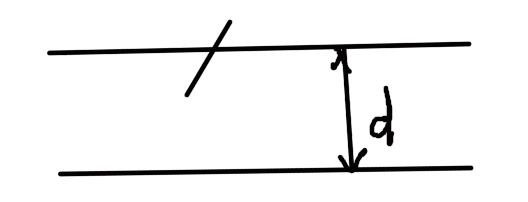
\includegraphics[width=5cm, height=4cm]{images/L09/buffon0.jpeg}
\caption{x}
\end{figure}

The needle can fall in one of two ways:

\begin{figure}[h]
\centering
\begin{minipage}{.45\linewidth}
  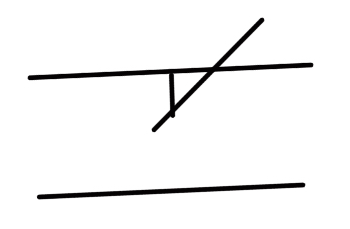
\includegraphics[width=\linewidth]{images/L09/buffon1.jpeg}
  \caption{Fall \#1}
  \label{bufffon1}
\end{minipage}
\hspace{.05\linewidth}
\begin{minipage}{.45\linewidth}
  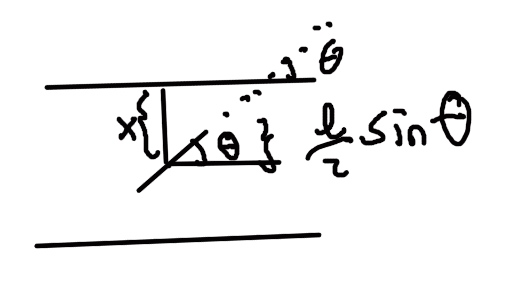
\includegraphics[width=\linewidth]{images/L09/buffon2.jpeg}
  \caption{Fall \#2}
  \label{bufffon2}
\end{minipage}
\end{figure}


\marginpar{(29m)}

Experimental measurement of Buffon's Needle problem.

\marginpar{(31m)}

Can interpret integral as a probability - simulation - Monte Carlo method

\subsection{Conditioning}

\marginpar{(31m)}

\subsection{Example: Stick-breaking}

\marginpar{(40:50m)}


\section{Lecture 10: Continuous Bayes' Rule; Derived Distributions}

\marginpar{\href{https://youtu.be/H_k1w3cfny8}{Video}}
\marginpar{\href{https://ocw.mit.edu/courses/6-041sc-probabilistic-systems-analysis-and-applied-probability-fall-2013/pages/unit-ii/lecture-10/}{Lecture Home}}
\marginpar{\href{https://ocw.mit.edu/courses/6-041sc-probabilistic-systems-analysis-and-applied-probability-fall-2013/b8c5d01b95379ca38ea3057529d253f7_MIT6_041SCF13_L10.pdf}{Slides}}

Reading: 3.6, 4.1

Conditional PDF's are just slices of joint PDF's

\subsection{The Bayes' Variations}

\marginpar{(4m)}

\begin{figure}[h]
\centering
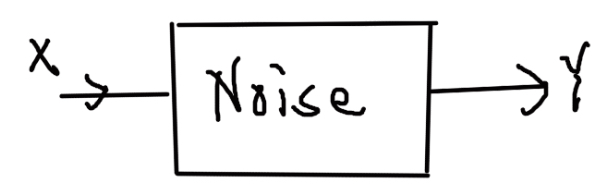
\includegraphics[width=6cm, height=3cm]{images/L10/noise_model.jpeg}
\caption{x}
\end{figure}

\marginpar{(5:45)}

The output of an inference problem is to come up with the distribution of X (unknown quantity) given what we observe.

\subsubsection{Continuous Counterpart}

\begin{align*}
f_{X|Y}(x|y) = \frac{f_{X,Y}(x,y)}{f_Y(y)}  = \frac{f_X(x) f_{Y|X}(y|x)}{f_Y(y)}\\
f_Y(y) = \int_X f_X(x) f_{Y|X}(y,x)dx
\end{align*}

\subsection{Discrete X, Continuous Y}

\marginpar{(10m)}

\begin{figure}[h]
\centering
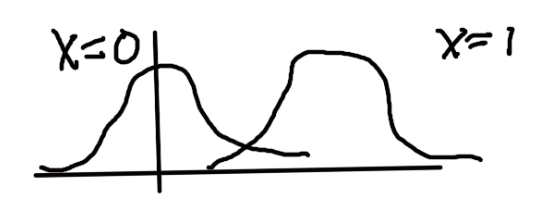
\includegraphics[width=5cm, height=4cm]{images/L10/discrete_continuous.jpeg}
\caption{Discrete X, Continuous Y}
\end{figure}

\subsection{Continuous X, Discrete Y}

\marginpar{(17:50)}

\begin{figure}[h]
\centering
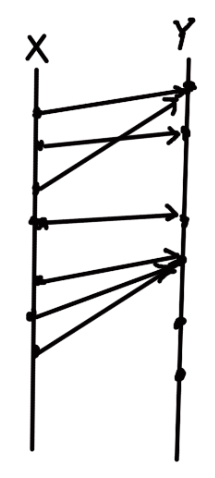
\includegraphics[width=4cm, height=8cm]{images/L10/continuous_discrete.jpeg}
\caption{Continuous X, Discrete Y}
\end{figure}

\subsection{Derived Distribution}

\marginpar{(20:30)}

\subsection{Discrete Case}

\marginpar{(22:45)}

\subsection{Continuous Case}

\marginpar{(23:45)}

\subsection{Two-step Procedure}

\marginpar{(26:10)}

\subsection{Example: Joan drives from Boston to NY}

\marginpar{(32:45)}

\begin{figure}[h]
\centering
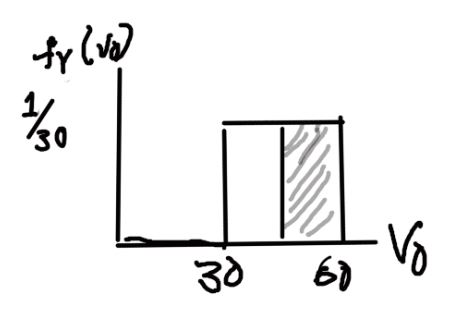
\includegraphics[width=5cm, height=4cm]{images/L10/joan_drives.jpeg}
\caption{x}
\end{figure}

\subsection{PDF of \texorpdfstring{$Y=aX + b$}{Y} }

\marginpar{(38:45)}

\subsection{\texorpdfstring{$a > 0$}{a}}

\marginpar{(43:50)}

\section{Lecture 11: Derived Distributions; Convolution; Covariance and Correlation}

\marginpar{\href{https://youtu.be/l4NoMKEHQwM}{Video}}
\marginpar{\href{https://ocw.mit.edu/courses/6-041sc-probabilistic-systems-analysis-and-applied-probability-fall-2013/pages/unit-ii/lecture-11/}{Lecture Home}}
\marginpar{\href{https://ocw.mit.edu/courses/6-041sc-probabilistic-systems-analysis-and-applied-probability-fall-2013/e4eb782ee3db745a86a3cef03d4c9e30_MIT6_041SCF13_L11.pdf}{Slides}}
Reading: 4.1, 4.2

How to derive the distribution of a function of a random variable.

$W=X+Y$ - shows up often

\begin{figure}[h]
\centering
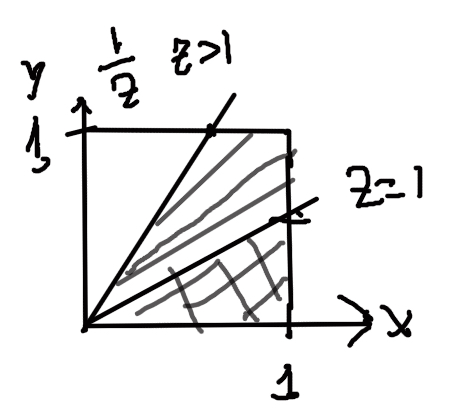
\includegraphics[width=5cm, height=4cm]{images/L11/derived_dist_z.jpeg}
\caption{$Z=g(X,Y)=\frac{Y}{X}$}
\end{figure}

Find PDF of $Z=g(X,Y)=\frac{Y}{X}$

\begin{align*}
F_z{z}=P \left(\frac{Y}{X} \le Z \right) = \frac{Z}{2},\quad Z le 1
\end{align*}

\begin{align*}
F_z{z}= 1 - \frac{1}{2}1\frac{1}{Z} = \frac{1}{2},\quad Z \ge 1\\
F_z{z}= 0, Z < 0
\end{align*}

\begin{align*}
E[Z] = \int_0^1 z \frac{1}{2}dz + \int_1^{\infty} \underbrace{z \frac{1}{2 z^2}dz}_{\infty}
\end{align*}
We get an infinite expectation.  That's nothing strange.

\marginpar{(13:25)}

A general formula: -don't need to go through cumulative.


Let $Y=g(X)$, g strictly monotonic

\marginpar{(18:20)}

$Y=X^3$, $g(X)=X^3 = y$
$X=y^\frac{1}{3}$

\begin{align*}
f_X(x)=f_{Y}(y)\cdot 3x^2
f_Y(y)=?
 = f_X(y^\frac{1}{3}) \cdot \frac{1}{3y^\frac{2}{3}}
\end{align*}

\marginpar{20:30)}

\begin{figure}[h]
\centering
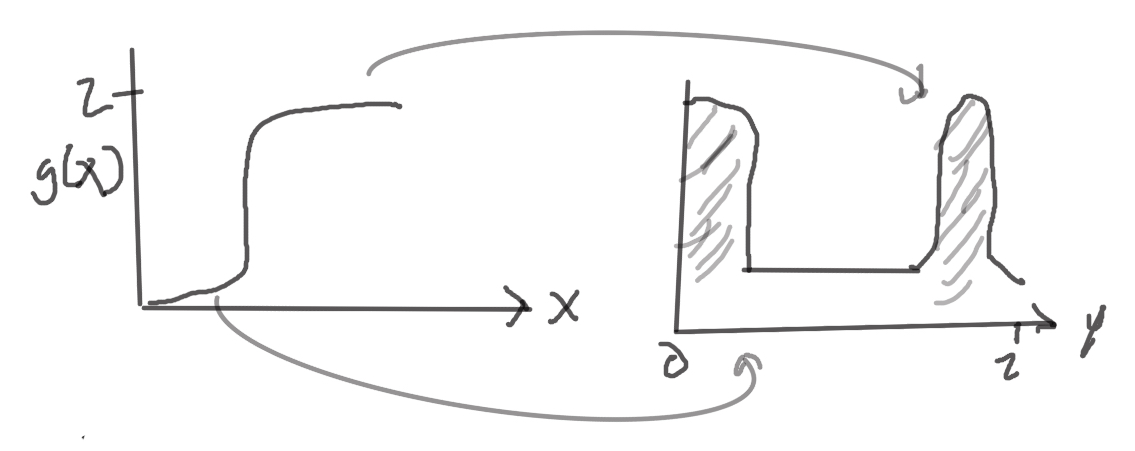
\includegraphics[width=6cm, height=4cm]{images/L11/strictly_monotonic.jpeg}
\caption{x}
\end{figure}

NOTE: y tales values close to zero. Flat $g()$ gives more density.

\subsection{Distribution of X+Y}

\marginpar{24:30)}

\begin{figure}[h]
\centering
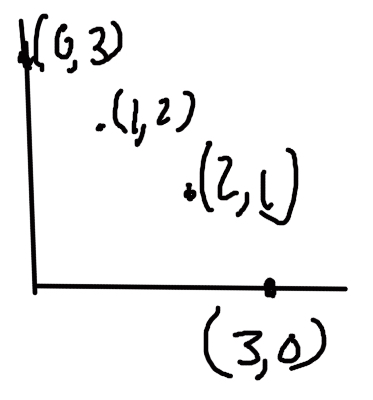
\includegraphics[width=6cm, height=4cm]{images/L11/dist_x_y.jpeg}
\caption{x}
\end{figure}

\subsection{Continuous Case}

\marginpar{31:50)}

Slide.

See derivation in text.

\subsection{Two Independent Normal RVs}

\marginpar{33:30)}

\begin{itemize}
    \item What does joint PDF look like?
    \item Ellipses, centered at $\mu_x, \mu_y$
\end{itemize}

\begin{figure}[h]
\centering
\begin{minipage}{.45\linewidth}
  
\includegraphics[width=\linewidth]{images/L11/wider.jpeg}
  \caption{$\sigma_x > \sigma_y$}
  \label{wider}
\end{minipage}
\hspace{.05\linewidth}
\begin{minipage}{.45\linewidth}
  
\includegraphics[width=\linewidth]{images/L11/taller.jpeg}
  \caption{$\sigma_x < \sigma_y$}
  \label{taller}
\end{minipage}
\end{figure}

\begin{figure}[h]
\centering
\includegraphics[width=6cm, height=4cm]{images/L11/percent_circle.jpeg}
\caption{$\sigma_x = \sigma_y$}
\end{figure}

\subsection{Sum of Independent Normal Random Variables}

\marginpar{39:20)}

$X \sim N(0, \sigma_x^2), \qquad Y \sim N(0, \sigma_y^2)$

Let $W=X+Y$.  The sum is also normal: $mean=0,var=\sigma_x^2 + \sigma_y^2$

\subsection{Covariance}

\marginpar{41:40)}

\begin{align*}
    cov(X,Y)=E[X-E[X]] - [Y - E[Y]] \\
    = E[XY] - E[X]E[Y]
\end{align*}

\begin{align*}
cov(X,X)=var(X)
\end{align*}

Covariance has the wrong units.

\subsection{Correlation Coefficient}

\marginpar{48m)}

\begin{align*}
\rho = \frac{cov(X,Y)}{\sigma_X \sigma_Y}, \qquad 0 \le \rho \le 1
\end{align*}
Removes units

$\rho$ is the correlation coefficient.

\section{Lecture 12: Iterated Expectations; Sum of a Random Number of Random Variables}

\marginpar{\href{https://youtu.be/P7a4bjE6Crk}{Video}}
\marginpar{\href{https://ocw.mit.edu/courses/6-041sc-probabilistic-systems-analysis-and-applied-probability-fall-2013/pages/unit-ii/lecture-12/}{Lecture Home}}
\marginpar{\href{https://ocw.mit.edu/courses/6-041sc-probabilistic-systems-analysis-and-applied-probability-fall-2013/e3e0a97e8298a57f911e24c304008870_MIT6_041SCF13_L12.pdf}{Slides}}

Reading: 4.3, 4.5 (no transforms)

This lecture is the end of the core material for the class (probability).

Conditional Expectations: $E[X|Y$
\begin{itemize}
    \item Law of Iterated Expectations
    \item Law of Total Variance
\end{itemize}

\subsection{Conditional Expectations}

\marginpar{1:38)}

\begin{align*}
    E[X|Y=y]= \sum_x x p_{X|Y}(x|y)
\end{align*}

\begin{align*}
    E[X|Y=y]=\frac{y}{2} \qquad (number)
\end{align*}

\begin{align*}
    E[X|Y=y]=\frac{Y}{2} \qquad (r.v.)
\end{align*}

\marginpar{7:55)}

\begin{align*}
    E[X|Y]=g(Y)\\
    E[X|Y=y]=g(y)\\
    E[E[X|Y]]=E[g(Y)]
\end{align*}

\begin{align*}
E[E[X|Y]]=E[X]
\end{align*}

\subsection{Law of Total Variance}
\marginpar{15:10)}

\begin{align*}
var(X) = E[var(X|Y)] + var(E[X|Y])
\end{align*}

Proof confusing and no intuition



\subsection{Baby Example}
\marginpar{19:30)}


\subsection{Example}
\marginpar{31m)}

\begin{figure}[h]
\centering
\includegraphics[width=6cm, height=4cm]{images/L11/percent_circlwww.jpeg}
\caption{x}
\end{figure}

\begin{align*}
var(X) = E[var(X|Y)] + var(E[X|Y]) \qquad (LOTV)
\end{align*}

\begin{align*}
E[X|Y=1] = \frac{1}{2}, \qquad E[X|Y=2] = \frac{3}{2}
\end{align*}

\begin{align*}
var(X|Y=1) = \frac{1}{2}, \qquad var(X|Y=2) = \frac{1}{2}
\end{align*}

\begin{align*}
var(E[X|Y]) = \frac{1}{3} \left(\frac{1}{2} - \frac{7}{6} \right)^2 + \frac{2}{3} \left( \frac{3}{2} - \frac{7}{6} \right)^2
\end{align*}

\subsection{Sum of Random Number of Independent Random Variables}

\marginpar{36m)}

\begin{itemize}
    \item N: \# stores visited
    \item $X_i$: money spent at store i. iid
\end{itemize}


Let $Y=X_1+ \cdots + X_n$

\begin{align*}
    E[Y|N=n] = slides...\\
    = nE[X]
\end{align*}

\subsection{Variance of Sum of Random Number of Independent Random Variables}

\marginpar{44m)}

slide...
EVE:
\begin{align*}
var(Y) = E[var(Y|N)] + var(E[Y|N])\\
 = E[N] var(X) + (E[X])^2 var(N)
\end{align*}

\section{Lecture 13: Bernoulli Process}

\marginpar{\href{https://youtu.be/gMTiAeE0NCw}{Video}} Reading: 6.1
\marginpar{\href{https://ocw.mit.edu/courses/6-041sc-probabilistic-systems-analysis-and-applied-probability-fall-2013/pages/unit-iii/lecture-13/}{Lecture Home}}

Stochastic processes - phenomenom that evolve over time.

\marginpar{(3:10)} 

\subsection{Bernoulli Process}

\begin{itemize}
    \item Sequence of independent Bernouilli trials
    \item At each i:
    \begin{itemize}
        \item $P(X_i=1)=p$
        \item $P(X_i=0)=1-p$
    \end{itemize}
\end{itemize}

\subsection{Random Process}

\marginpar{(6:50)} 

\begin{itemize}
    \item Two views:
    \begin{itemize}
        \item Sequence of RVs
        \item What is the right sample space?  One long experiment.
    \end{itemize}
\end{itemize}


Random Process we study:
\begin{itemize}
    \item Bernoulli process - memoryless, discrete
    \item Poisson process - memoryless, continuous
     \item Markov chains - with memory/dependence across time
\end{itemize}

\marginpar{(18:30)} 

\section{Lecture 14: Poisson Process - I}

\marginpar{\href{https://youtu.be/jsqSScywvMc}{Video}}
\marginpar{\href{https://ocw.mit.edu/courses/6-041sc-probabilistic-systems-analysis-and-applied-probability-fall-2013/pages/unit-iii/lecture-14/}{Lecture Home}}

Reading: 6.2

\begin{itemize}
    \item success - something arrives
    \item failure - nothing arrives
\end{itemize}

\subsection{Poisson Process}

\marginpar{(9:10)} 

\subsection{Example: Email Arrival Rate}

\marginpar{(29:15)}

\subsubsection{Erlang Distribution}


\subsection{Bernoulli/Poisson Relationship}

\marginpar{(42:10)}

\begin{table}[ht]
    \centering
    \begin{tabular}{c|c|c}
           & Poisson & Bernoulli \\
           \hline \\
         Inter-arrival distance & Exponential & Geometric  \\
         \hline \\
         Time to k-th arrival & Erlang & Pascal PMF 
    \end{tabular}
    \caption{Caption}
    \label{tab:Poisson_Bernoulli_label}
\end{table}

\marginpar{(43:20)}

\begin{table}[]
    \centering
    \begin{tabular}{c|c| c}
         & Green Flashes & Green does not \\
         \hline \\
         Red flashes&  &\\
         \hline \\
         Red does not & & 
    \end{tabular}
    \caption{Caption}
    \label{tab:red_flashes_label}
\end{table}
\section{Lecture 15: Poisson Process - II}

\marginpar{\href{https://youtu.be/XsYXACeIklU}{Video}}
\marginpar{\href{https://ocw.mit.edu/courses/6-041sc-probabilistic-systems-analysis-and-applied-probability-fall-2013/pages/unit-iii/lecture-16/}{Lecture Home}}

Review 
\begin{itemize}
    \item Time homogeneity $P(k, \tau) - \Sigma = 1$
    \item Independence
    \item Small interval probabilities  (small $\delta)$
\end{itemize}

\begin{align*}
P(k,\delta)=
\begin{cases}
    1 - \lambda \delta, \qquad k=0\\
    \lambda \delta, \qquad k=1\\
    0, \qquad, k>1
\end{cases}    
\end{align*}

\marginpar{(7:20)}  Another way of thinking about the Poisson process: Let things evolve over time.

Light bulb - used bulb is exactly as good as new.

\subsection{Example: Poisson Fishing}

\marginpar{(7:20)}

Fish caught according to Poisson process: $\lambda=0.6/hour$

\begin{itemize}
    \item Fish for 2 hours
    \item If nothing caught, continue until first catch
\end{itemize}

\begin{itemize}
    \item $P(\text{fish for} > 2hours) = $
    \item $P(\text{fish for} > 2hours and < 5) = $
    \item $P(\text{catch at least 2 fish}) = $
    \item $E[\# fish]=$
    \item E[future fishing time | fished for 4 hours] =
    \item E[total fishing time] = 
\end{itemize}

\subsection{Review Merging Poisson Processes}

\marginpar{(21:40)}

\subsection{Example: Light bulb}

\marginpar{(26:40)}

\subsection{Splitting of Poisson Processes}


\subsection{Random Incidence for Poisson Processes}

\subsection{Random Incidence in "Renewal Processes"}

Was your bus empty? No witnesses on empty bus.

\section{Lecture 16: Markov Chains - I}

\marginpar{\href{https://youtu.be/IkbkEtOOC1Y}{Video}}

\marginpar{\href{https://ocw.mit.edu/courses/6-041sc-probabilistic-systems-analysis-and-applied-probability-fall-2013/pages/unit-iii/lecture-16/}{Lecture Home}}
\marginpar{\href{https://ocw.mit.edu/courses/6-041sc-probabilistic-systems-analysis-and-applied-probability-fall-2013/290daad9889bbffb3b9c1c29f5028f98_MIT6_041SCF13_L16.pdf}{Slides}}

Reading: 7.1, 7.2\\

new state = f(old state, noise)

\subsection{Checkout Counter Model}

\marginpar{(2:45)}

\subsection{Finite State Markov Chains}

\marginpar{(11:30)}

% \subsection{Finite State Markov Chains}

% \marginpar{(11:30)}

\subsection{n-step Transition Probabilities}

\marginpar{(20:10)}

\begin{align*}
    r_{ij} = P(X_n=j|X_0 = i)
\end{align*}

Key recursion
\begin{align*}
    r_{ij}(n) = \sum_{k=1}^m r_{ik}(n-1)r_{kj}, % \foreach_{i,j}
\end{align*}

\subsection{Example}

\marginpar{(28:25)}

\begin{figure}[ht]
\centering
	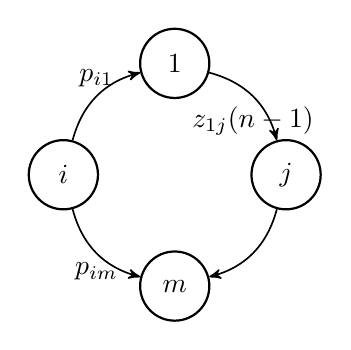
\begin{tikzpicture}[->, >=stealth', auto, semithick, node distance=2cm]
	\tikzstyle{every state}=[fill=white,draw=black,thick,text=black,scale=1]
	\node[state]    (A)                     {$i$};
	\node[state]    (B)[above right of=A]   {$1$};
    \node[state]    (D)[below right of=A]   {$m$};
     \node[state]   (C)[below right of=B]   {$j$};
	\path
	(A) 
      edge[bend left,above] node{$p_{i1}$} (B)
      edge[bend right,below] node{$p_{im}$} (D)
    (B) 
	edge[bend left,below]	node{$z_{1j}(n-1)$}	(C)
    (C) edge[bend left,below]	node{}	(D)
 ;
	\end{tikzpicture}
\end{figure}

\begin{align*}
 &r_{11}(n) = r_{1,2}(n-1) \cdot + r_{1,1}(n-1)\cdot 0.5 \\
 &r_{12}(n) = 1 - r_{11}(n)
\end{align*}

\marginpar{(30:30)}

\begin{figure}[ht]
\centering
	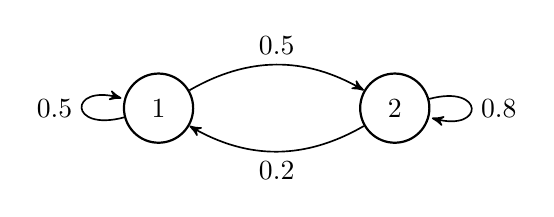
\begin{tikzpicture}[->, >=stealth', auto, semithick, node distance=3cm]
	\tikzstyle{every state}=[fill=white,draw=black,thick,text=black,scale=1]
	\node[state]    (A)                     {$1$};
	\node[state]    (B)[right of=A]   {$2$};
	\path
	(A) edge[loop left]			node{$0.5$}	(A)
      edge[bend left,above] node{$0.5$} (B)
    (B) edge[loop right]			node{$0.8$}	(B)
	edge[bend left,below]	node{$0.2$}	(A);
	\end{tikzpicture}
\end{figure}


\begin{table}[]
    \centering
    \begin{tabular}{c|c|c|c|c|c|}
         & n=0 & n=1 & n=2 & n=100 & n=101 \\
         \hline 
         $r_{11}(n)$& 1 & 0.5 & 0.35 & $\approx \frac{2}{7}$ & $\approx \frac{2}{7}$\\
         $r_{12}(n)$& 0 & 0.5 & 0.65 & $\approx \frac{5}{7}$ & $\approx \frac{5}{7}$\\
         $r_{21}(n)$& 0 & 0.2 &   & $\approx \frac{2}{7}$ &\\
         $r_{22}(n)$& 1 & 0.8 &   & $\approx \frac{5}{7}$ &\\   
    \end{tabular}
    \caption{Caption}
    \label{tab:my_label}
\end{table}

The state of the chain doesn't care about the initial state.

\subsection{Generic Convergence Questions}

\marginpar{(41m)}

\begin{itemize}
    \item Does $r_{ij}(n)$ converge to something?
    \item Can fail if chain has a periodic structure. \textbf{Periodicity}
    \item Does the limit depend on the initial state?
\end{itemize}

\subsection{Recurrent and Transient States}

\marginpar{(47:30)}


\section{Lecture 17: Markov Chains - II}

\marginpar{\href{https://youtu.be/ZulMqrvP-Pk}{Video}}
\marginpar{\href{https://ocw.mit.edu/courses/6-041sc-probabilistic-systems-analysis-and-applied-probability-fall-2013/pages/unit-iii/lecture-17/}{Lecture Home}}
\marginpar{\href{https://ocw.mit.edu/courses/6-041sc-probabilistic-systems-analysis-and-applied-probability-fall-2013/0c0f13321d15596341420d11ce07fcc7_MIT6_041SCF13_L17.pdf}{Slides}}

\subsection{Recurrent and transient states}


\subsection{Periodic States}


\subsection{Steady-State Probabilities}


\subsection{Visit frequency interpretation}


\subsection{Example}


\subsection{Birth-death processes}



\section{Lecture 18: Markov Chains - III}

\marginpar{\href{https://youtu.be/HIMxdWDLEK8}{Video}}
\marginpar{\href{https://ocw.mit.edu/courses/6-041sc-probabilistic-systems-analysis-and-applied-probability-fall-2013/pages/unit-iii/lecture-18/}{Lecture Home}}
\marginpar{\href{https://ocw.mit.edu/courses/6-041sc-probabilistic-systems-analysis-and-applied-probability-fall-2013/3dd39ef98a1da35dbe78dfbd702a4748_MIT6_041SCF13_L18.pdf}{Slides}}



\subsection{Review}


\subsection{Example}


\subsection{phone company proble}


\subsection{Calculating absorption probabilities}


\subsection{Expected time to absorption}

\subsection{Mean first passage and recurrence times}



\section{Lecture 19: Weak Law of Large Numbers}

\marginpar{\href{https://youtu.be/3eiio3Tw7UQ}{Video}}
\marginpar{\href{https://ocw.mit.edu/courses/6-041sc-probabilistic-systems-analysis-and-applied-probability-fall-2013/pages/unit-iv/lecture-19/}{Lecture Home}}
\marginpar{\href{https://ocw.mit.edu/courses/6-041sc-probabilistic-systems-analysis-and-applied-probability-fall-2013/d569abb143b22f469a09ff218cb3383c_MIT6_041SCF13_L19.pdf}{Slides}}
Reading: 5.1-5.3, Start 5.4
\\
Introducing limit theorems\\

Collect n samples:  $X_1,\ldots, X_n$, iid.

This is the estimate of your expected value:
\begin{align*}
    M_n = \frac{X_1 +\cdots + X_n}{n}, \qquad \text{Sample mean of collected data}
\end{align*}

\marginpar{(\href{https://youtu.be/3eiio3Tw7UQ?t=2m}{(2:00)}} Expected value $E[X]$ is the mean over the entire population.  It is a number.
The sample mean is a random variable because the sample you have collected is random.

\subsection{Markov Inequality}

\marginpar{\href{https://youtu.be/3eiio3Tw7UQ?t=5m35s}{(5:35)}}

Take a non-negative discrete RV: $X \ge 0$, $E[X] = \sum_x x p_X(x)$

Since we are adding non-negative,  summing fewer things gives us a smaller values

Restrict x to be greater than some constant; (i.e. removing values}
\begin{align*}
    E[X] = \sum_x x p_X(x) \ge \sum_{x\ge a} x p_X(x), 
\end{align*}

\marginpar{\href{https://youtu.be/3eiio3Tw7UQ?t=6m50s}{(6:50)}} Now a becomes a constant that we can pull outside the summation:
\begin{align*}
    \mathbb{E}[X] = \sum_x x p_X(x) \ge \sum_{x\ge a} x p_X(x) \ge  \sum_{x \ge a} a p_X(x) \ge a \sum_{x\ge a} p_X(x) = a P(X \ge a)
\end{align*}

We have arrived at the Markov inequality.  It relates expected values to probabilities.  If the expected value is small then probability that X is big is also small.

We need this statement but in a different form.

\marginpar{\href{https://youtu.be/3eiio3Tw7UQ?t=6m50s}{(6:50)}}

\begin{align*}
&\mu = E[X]\\
&    \underbrace{E[(X - \mu)^2]}_{Variance} \ge P((X - \mu)^2 \ge a^2) a^2
\end{align*}

\marginpar{\href{https://youtu.be/3eiio3Tw7UQ?t=9m45s}{(9:45)}} This relates the variance of X to the probability of being far away from the mean is also small.

\subsection{Chebyshev’s inequality}

\marginpar{Slide: Chebyshev’s inequality}

Now we do a continuous case where we choose a big number to integrate far away from the mean.

\marginpar{\href{https://youtu.be/3eiio3Tw7UQ?t=12m35s}{(12:35)}} The variance is the spread of the distribution. If the variance is small the distribution is not very wide.  This translate mathematically, when the variance is small, the probability of being far away from the mean is small.

Instead of using c, we think of the value as $k\cdot \sigma$.  This is the event that we are k standard deviations away from the mean.

The Chebyshev inequality comes in handy whenever you want to relate probabilities and expected values.  This tells you something about tail probabilities.

\subsection{Deterministic limits}

\marginpar{Slide: Deterministic limits}

\marginpar{\href{https://youtu.be/3eiio3Tw7UQ?14m30s}{(14:30)}}

\begin{figure}[ht]
\centering
\includegraphics[width=7cm, height=4cm]{images/L19/IMG_3316.jpeg}
\caption{Convergence of a Sequence}
\end{figure}

\marginpar{\href{https://youtu.be/3eiio3Tw7UQ?16m20s}{(16:20)}}Convergence means given a band of positive length around the number a, the values of the sequence that you get, eventually stay inside the band.  This holds no matter how narrow the band is made to be.

\subsection{Convergence "in probability"}

\marginpar{\href{https://youtu.be/3eiio3Tw7UQ?17m50s}{(17:50)}}
\marginpar{Slide: Convergence "in probability"}

What does it mean for a sequence of random variables to converge to a number?

\marginpar{\href{https://youtu.be/3eiio3Tw7UQ?18m30s}{(18:30)}} Now we want the distribution inside the band.  The tails won't be, but we want more and more.

\begin{figure}[ht]
\centering
\includegraphics[width=7cm, height=4cm]{images/L19/IMG_3317.jpeg}
\caption{Convergence of RV}
\end{figure}

The mathematical statement is messy...better to think of the bands analogy.

\subsubsection*{Example}

\marginpar{\href{https://youtu.be/3eiio3Tw7UQ?22m00s}{(22:00)}}

\begin{figure}[ht]
\centering
\includegraphics[width=7cm, height=4cm]{images/L19/IMG_1572.jpeg}
\caption{Does $Y_n converge?$}
\end{figure}

$Y_n$ converges in probability to zero.
What is the $\mathbb{E}[Y_n]$

\begin{align*}
    \mathbb{E}[Y_n] = n\cdot\frac{1}{n} = 1
\end{align*}

\begin{align*}
    \mathbb{E}[Y_n^2] = \infty
\end{align*}

\marginpar{\href{https://youtu.be/3eiio3Tw7UQ?24m00s}{(24:00)}} Convergences of a RV to zero doesn't imply anything about  convergence expected value, variance, etc.  It doesn't tell us how far the tail goes.

\subsection{Convergence of the Sample Mean}

\marginpar{\href{https://youtu.be/3eiio3Tw7UQ?25m00s}{(25:00 - Slide)}}

\begin{align*}
    M_n = \frac{X_1 + \cdots + X_n}{n} = \text{Sample Mean}
\end{align*}

\begin{align*}
    \mathbb{E}[M_n] = \frac{E[X_1] + \cdots + E[X_n]}{n} = \frac{n \mu}{n} = \mu
\end{align*}

\marginpar{\href{https://youtu.be/3eiio3Tw7UQ?27m00s}{(27:00)}} The sample mean is the heights we collected over a single expedition; this is $M_n$.  The expected value means thinking over a huge number of expeditions.  We average the averages at each expedition: $E[M_n]$.  Remember expectations always give numbers, where as the sample mean is a random variable.

\begin{align*}
    Var(M_n) = \frac{n \cdots \sigma^2}{n^2} = \frac{\sigma^2}{n}
\end{align*}
The variance of the sample mean becomes smaller and smaller.

Having a large sample size removes the randomness from the experiment.

Let's apply the Chebyshev inequality to say something about the tail probabilities for the sample mean.

The probability that you are more than $\varepsilon$ away from the true mean is less than or equal to $Var(M_n)/\varepsilon^2$:

\begin{align}
    P(|M_n - \mu| \ge \varepsilon) \le \frac{Var(M_n}{\varepsilon^2} = \frac{\sigma^2}{n \varepsilon^2}
\end{align}

We have convergence \emph{in probability} to the sample mean to the true mean.

\subsection{Example: The Pollster’s Problem}

\marginpar{\href{https://youtu.be/3eiio3Tw7UQ?30m45s}{(30:45)}}

Slide: The pollster’s problem\\

\marginpar{\href{https://youtu.be/3eiio3Tw7UQ?36m30s}{(36:30)}}
\begin{figure}[ht]
\centering
\includegraphics[width=7cm, height=4cm]{images/L19/IMG_3318.png}
\caption{$p(1-p)$}
\end{figure}

We are going to use the worst value for $\sigma_X^2$, which is 4.

Solving for n, we find that it needs to be greater than or equal to 50,000.

\marginpar{\href{https://youtu.be/3eiio3Tw7UQ?38m40s}{(38:40)}}

50,000 is too many people to sample so we try to cut corners.  Newspapers will go with $\pm$3 percentage points instead of 1 point.  This saves you a factor of 10.  Chebyshev is not a very tight inequality.  It's not that accurate.

\subsection{Different scalings of \texorpdfstring{$M_n$}{M}}

\marginpar{\href{https://youtu.be/3eiio3Tw7UQ?40m00s}{40:00)}}

Slide: Different scalings of $M_n$

\begin{figure}[ht]
\centering
\includegraphics[width=7cm, height=4cm]{images/L19/IMG_3319.jpeg}
\caption{Scaling vs No Scaling}
\end{figure}

We decide to divide the sum by $\sqrt{n}% instead of n.

\begin{figure}[ht]
\centering
\includegraphics[width=7cm, height=4cm]{images/L19/IMG_3320.jpeg}
\caption{Eqn}
\end{figure}

\begin{align}
    Var()=
\end{align}

So, when we scale in this particular way $S_n$ changes but the variance doesn't change.

\subsection{Central Limit Theorem}

\marginpar{\href{https://youtu.be/3eiio3Tw7UQ?38m40s}{(44:10)}}

Slide: Central Limit Theorem\\



\section{Lecture 20: Central Limit Theorem}

\marginpar{\href{https://youtu.be/Tx7zzD4aeiA}{Video}}

\marginpar{\href{https://ocw.mit.edu/courses/6-041sc-probabilistic-systems-analysis-and-applied-probability-fall-2013/pages/unit-iv/lecture-20/}{Lecture Home}}

\marginpar{\href{https://ocw.mit.edu/courses/6-041sc-probabilistic-systems-analysis-and-applied-probability-fall-2013/e2d51b7d3f67afbc118dbb3478276ec5_MIT6_041SCF13_L20.pdf}{Slides}}

Reading: 5.4

\subsection{Theorem}


\subsection{Normal Approximation}

\subsection{Example: Pollster’s problem using the CLT}


\subsection{Apply to binomial}


\subsection{The 1/2 correction for binomial approximation}



\subsection{De Moivre–Laplace CLT}


\subsection{Poisson vs. normal approximations of the binomial}



\section{Lecture 21: Bayesian Statistical Inference - I}

\marginpar{\href{https://youtu.be/1jDBM9UM9xk}{Video}}

\marginpar{\href{https://ocw.mit.edu/courses/6-041sc-probabilistic-systems-analysis-and-applied-probability-fall-2013/pages/unit-iv/lecture-21/}{Lecture Home}}

\marginpar{\href{https://ocw.mit.edu/courses/6-041sc-probabilistic-systems-analysis-and-applied-probability-fall-2013/e581867107d8494749a2ced11ad812ff_MIT6_041SCF13_L21.pdf}{Slides}}

Reading: 8.1-8.2

\subsection{Types of Inference models}


\subsection{Bayesian inference: Use Bayes rule}


\subsection{Estimation with discrete data}


\subsection{Output of Bayesian Inference}


\subsection{Least Mean Squares Estimation}


\subsection{LMS Estimation of $\Theta$ based on X}


\section{Lecture 22: Bayesian Statistical Inference - II}

\marginpar{\href{https://youtu.be/XtNXQJkgkhI}{Video}}

\marginpar{\href{https://ocw.mit.edu/courses/6-041sc-probabilistic-systems-analysis-and-applied-probability-fall-2013/pages/unit-iv/lecture-22/}{Lecture Home}}
\marginpar{\href{https://ocw.mit.edu/courses/6-041sc-probabilistic-systems-analysis-and-applied-probability-fall-2013/6b546ad68aa67f323597de2c688298d2_MIT6_041SCF13_L22.pdf}{Slides}}

\subsection{Conditional mean squared error}


\subsection{Properties of LMS Estimation}

\subsection{Linear LMS}

\subsubsection{Linear LMS properties}



\section{Lecture 23: Classical Statistical Inference - I}

\marginpar{\href{https://youtu.be/4UJc0S8APm4}{Video}}
\marginpar{\href{https://ocw.mit.edu/courses/6-041sc-probabilistic-systems-analysis-and-applied-probability-fall-2013/pages/unit-iv/lecture-23/}{Lecture Home}}
\marginpar{\href{https://ocw.mit.edu/courses/6-041sc-probabilistic-systems-analysis-and-applied-probability-fall-2013/6e8de3b1fae4b6dd8b6a677c70fd90b8_MIT6_041SCF13_L23.pdf}{Slides}}

\subsection{Classical statistics}

\subsection{Maximum Likelihood Estimation}

\subsection{Estimate a mean}

\subsection{Confidence intervals (CIs)}


\subsection{The case of unknown sigma}


\section{Lecture 24: Classical Statistical Inference - II}

\marginpar{\href{https://youtu.be/tBUHRpFZy0s}{Video}}

\marginpar{\href{https://ocw.mit.edu/courses/6-041sc-probabilistic-systems-analysis-and-applied-probability-fall-2013/pages/unit-iv/lecture-24/}{Lecture Home}}
\marginpar{\href{https://ocw.mit.edu/courses/6-041sc-probabilistic-systems-analysis-and-applied-probability-fall-2013/resources/mit6_041scf13_l24/}{Slides}}

\subsection{Review: Maximum likelihood estimation}


\subsection{\texorpdfstring{$1 - \alpha$}{1-a} Confidence Interval}

\subsection{Regression}

\subsection{Linear Regression}


\subsection{Binary Hypothesis Testing}


\subsection{Likelihood ratio test (LRT)}




\section{Lecture 25: Classical Statistical Inference - III}

\marginpar{\href{https://youtu.be/rYefUsYuEp0}{Video}}
\marginpar{\href{https://ocw.mit.edu/courses/6-041sc-probabilistic-systems-analysis-and-applied-probability-fall-2013/pages/unit-iv/lecture-25/}{Lecture Home}}
\marginpar{\href{https://ocw.mit.edu/courses/6-041sc-probabilistic-systems-analysis-and-applied-probability-fall-2013/6c879ec7e72ba6921b395b529b4c6eb0_MIT6_041SCF13_L25.pdf}{Slides}}

\subsection{Simple binary hypothesis testing}

\subsection{Example: Test on normal mean}

\subsection{Example: Test on normal variance}

\subsection{Composite hypotheses}

\subsection{Example: Is my die fair?}

\subsection{Do I have the correct pdf?}



\end{document}
